\chapter{Extended Source Detection above 50 GeV: The 2FHL Catalog}
\label{chap:2FHL}
\jamie{chage ROI to RoI}

\jamie{Application of addSrcs searching for extended (and really point too) sources in the sky. 2FHL results on all Galactic sources. Index histograms for entire \twofhl population showing harder index for Galactic sources.}

\jamie{we don't just detect extended though! The pipeline was built to try extended and if that's not likely, revert to point source. Simple check with Alberto's pipeline to show we didn't detect any glaring discrepancies. Quick check of Alberto's results for clusters of point source at \blat.}

\section{Introduction}\label{2FHL:intro}
\jamie{give this a different title
	}
The \lat{} \citep{atwood09} on board the \Fermi{}
\gam{} space telescope has been surveying the whole sky since August 2008.
Its unprecedented sensitivity and localization accuracy allowed the detection
of over 3,000 point-like sources in  4\,years of data \citep[see the
third catalog of {\it Fermi}-LAT sources, 3FGL, ][]{3FGL}.
Typically, {\it Fermi}-LAT catalog studies are based on  source detection
and characterization in the whole 0.1\,GeV--100\,GeV energy band.
The larger photon statistics present at low energy, counterbalanced by
the LAT point-spread function (PSF) whose size decreases with energy,
yields an optimum sensitivity at few-GeV energies.
The {\it Fermi}-LAT catalogs are thus representative of the GeV sky
more than they are of the MeV or the sub-TeV sky.


The first {\it Fermi}-LAT catalog of hard sources, named 1FHL \citep{1FHL}, provided an unbiased census of the sky at energies from 10~GeV up to 500~GeV. %The comparison of 1FHL and 0.1--100\,GeV observations \citep[as provided in][]{2FGL} allowed us to uncover the presence of spectral breaks and to determinethat  blazars of the BL Lacertae (BL Lac) type represented about 50\,\%of the entire source population { detected in that band}.
{ All-sky surveys at $\gamma$-ray energies} are instrumental for ground-based imaging atmospheric Cherenkov telescopes (IACTs) such as H.E.S.S., MAGIC, and VERITAS \citep[][respectively]{holder08,lorenz04,hinton04}
in order to find new sources because of their limited fields of view (FoV).


Recently, a new event-level  analysis (known as Pass 8) has been developed by the \emph{Fermi}-LAT collaboration \citep{atwood13b,atwood13}. Pass~8 significantly improves the LAT's background rejection, PSF, and effective area. All these  enhancements lead to a significant increase of the LAT sensitivity and its effective energy range, from below 100~MeV to beyond a few hundred GeV  \citep{atwood13b,atwood13}. These improvements are particularly significant above 50\,GeV, yielding an enhancement in the acceptance and PSF by a factor  between 1.2 and 2. 
It is interesting to note that, above 50\,GeV, both the PSF (governed mostly by the pitch of the tracker silicon strips and the spacing of the tracker planes, see Chapter \ref{FGST:LAT}) and the effective area of the LAT are only weakly dependent on energy and that the LAT 
operates, due to the (almost complete) absence of background, in the photon-limited regime.

We use 80\,months of Pass~8 data to produce a catalog of sources detected by the LAT at energies\footnote{Note the different energy range with respect to the 1FHL.} between 50\,GeV and 2\,TeV. This constitutes the second catalog of hard \lat sources, named \twofhl{}, which allows a thorough study of the properties of the whole sky in the sub-TeV domain. In this thesis, we present results published in \cite{2FHL}, exclusively focusing on the Galactic science analysis and results and eschew the extragalactic results to the published \twofhl{} paper.


%%%%%%%%%%%%%%%%%%%%%%%%%%%%%%%%%%%%%%%%%%%%%%%%%%%%%%%%%%%%%%%%
%
%         Analysis 
%
%%%%%%%%%%%%%%%%%%%%%%%%%%%%%%%%%%%%%%%%%%%%%%%%%%%%%%%%%%%%%%%%
\section{Analysis}
\label{sec:analysis}


%%%%%%%%%%%%%%%%%%%%%%%%%%%%%%%%%%%%%%%%%%%%%%%%%%%%%%%%%%%%%%%%
%
%         Detection
%
%%%%%%%%%%%%%%%%%%%%%%%%%%%%%%%%%%%%%%%%%%%%%%%%%%%%%%%%%%%%%%%%
% \subsection{\label{sec:sourceDetect}Data Selection and Source Detection}

\subsection{\label{sec:data_sel}Data Selection}


We use 80 months (from August 2008 to April 2015) of P8\_SOURCE 
photons with reconstructed energy in the 50\,GeV--2\,TeV range.
At these energies the LAT has an energy resolution of around 10--15\,\% (1\,$\sigma$).
Photons detected at zenith angles larger than 105$^{\circ}$ were excised
to limit the contamination from $\gamma$-rays generated by cosmic-ray
interactions in the upper layers of the atmosphere. Moreover, data were filtered
removing time periods when the instrument was not in sky-survey mode\footnote{This
	was achieved using the expression `(DATA\_QUAL$>$0)\&\&(LAT\_CONFIG==1)' in {\tt gtmktime}.}.
This leaves
approximately 61,000 photons detected all over the sky. The count map
reported in Figure~\ref{fig:skymap} shows that the \lat{} observes
many point-like sources and
large scale diffuse emission in the direction of our Galaxy, some of which appears
coincident  with the so-called {\it Fermi} bubbles \citep{su10,lat_bubbles}.



\begin{figure*}[!ht]
	\begin{centering} 
		\includegraphics[scale=0.85]{Figures/all-sky_countmap-Marco.eps}
		\caption{Adaptively smoothed count map in the 50\,GeV--2\,TeV band represented in Galactic coordinates and Hammer-Aitoff projection. The image has been smoothed with a Gaussian kernel whose size was varied to achieve a minimum signal-to-noise ratio under the kernel of 2. The color scale is logarithmic and the units are counts per (0.1\,deg)$^2$.
			\label{fig:skymap}}
	\end{centering}
\end{figure*}


\subsection{\label{2fhl:sourceDetect}Source Detection}


The first step of the source detection stage comprises the identification of source seeds, which are locations of potential sources whose significance is later tested through a maximum likelihood (ML) analysis. The seed detection method, described further in \cite{2FHL}, includes all the point sources detected in the 1FHL catalog. We note that  this seed list may include statistical fluctuations as well as real sources with a non-optimal position.

A full ML analysis is then performed in order to verify which,
among the seeds, are the reliable sources. 
The analysis is performed in 154 \rois{}, varying between 10$^{\circ}$ and 20$^{\circ}$ in radius, whose sizes and positions in the sky are optimized to cover all the seeds, ensuring that no more than 45 seeds are contained in a single \roi{}.
For each \roi{}, we build
a sky model that includes all the potential sources in the region
as well as the  Galactic and isotropic diffuse emissions\footnote{We~use~the~{\tt gll\_iem\_v06.fits}~and~{\tt iso\_P8R2\_SOURCE\_V6\_v06.txt}
	templates available at \\
	http://fermi.gsfc.nasa.gov/ssc/data/access/lat/BackgroundModels.html.}.
These models, which are defined only up to $\sim$600\,GeV and  $\sim$900\,GeV respectively, where extrapolated up to 2\,TeV.
The \roi{} models include also the extended sources present in the region (see Chapter \ref{2fhl:extended}).
The model is fit to the data via the unbinned ML algorithm provided
within the {\it Fermi} Science Tools\footnote{Available at 
	http://fermi.gsfc.nasa.gov/ssc/data/analysis/software/.} (version v9r34p3).

The spectrum of each source is modeled with a power law because
none of the sources is expected to show statistically
significant spectral
curvature detectable by the LAT in this energy band. 
Indeed, this was the case for the sources in the 1FHL catalog \citep{1FHL}.

The fit is performed iteratively in order to ensure convergence and 
to produce an optimal solution. It proceeds as follows:

\begin{enumerate}
	\item Complex ML fits require approximate knowledge of the 
	starting values of the parameters. For this reason the first
	step  aims to find those values  by fitting each single source separately 
	to determine approximate spectral parameters.
	Throughout the entire process, the parameters of the diffuse emission
	models are left free to vary.
	The significance of each source is evaluated using the test statistic  
	${\rm TS}=2(\ln \mathcal{L}_1 - \ln \mathcal{L}_0)$, where $\mathcal{L}_0$ and $\mathcal{L}_1$
	are the likelihoods of the background (null hypothesis) and 
	the hypothesis being tested (\eg source plus background). 
	At each step in the procedure, marginal sources, those with TS$ ~<$ 10, are removed from the model.
	Once the spectral parameters and significance of each source have
	been evaluated, a global fit for which all the parameters of the sources
	with a ${\rm TS}\geq 10$ are allowed to  vary is performed. 
	Then one more global fit is performed after removing all the sources that had ${\rm TS}< 10$ at the previous global fit.
	This step,
	as well as all the others, includes sources that
	are spatially extended (see Chapter \ref{2fhl:extended});
	
	\item In this second step, the positions of point-like sources, using the best-fit sky model
	derived at step 1, are optimized using the {\tt gtfindsrc} tool. This step
	is done iteratively as well by optimizing first the positions of the
	most significant sources found at step 1 and later  those of the fainter
	ones;
	
	\item The parameters and significances of sources are estimated again (as in step 1) using the best-fit source positions. This step produces the best-fit sky 
	model for any given \roi{}. 
	Seeds with $10\leq {\rm TS}<25$ are included in the model, but not reported in the final catalog;
	
	\item For each source we estimate the energy of the \hep{}
	that the fit attributes robustly  to the source model. This is done using the tool {\tt gtsrcprob} and selecting the HEP that has a probability $>85$\,\% to belong to the source;
	
	\item A  spectrum with three logarithmically spaced bins (boundaries of 50\,GeV, 171\,GeV, 585\,GeV, 2\,TeV) is generated for each source in the \roi{} that is detected with ${\rm TS}\geq 25$ and with the number of detected $\gamma$ rays (estimated by the likelihood, N$_{\rm pred}$) to be $\geq$3.
	
	
\end{enumerate}

The procedure described above achieves the detection of 360 sources (including
the extended sources discussed next at Chapter \ref{2fhl:extended}) 
with TS $\geq$ 25 and N$_{\rm pred}\geq3$ across the entire sky.
The number of seeds kept in the ROI models
with $10\leq{\rm TS}<25$ is 453, while 7 are the seeds with ${\rm TS\geq}25$, but N$_{\rm pred}<3$.
\jamie{took out the monte carlo sims reasoning for Npred}
%We have performed seven Monte Carlosimulations of the $>$50\,GeV sky whose data have been analyzed like the real data (as detailed above). The  N$_{\rm pred}$ cut was introducedon the basis of these simulations to limit to $\lesssim$1\,\% the number of false positives in the final catalog. These simulations will be discussed in a forthcoming publication.

%%%%%%%%%%%%%%%%%%%%%%%%%%%%%%%%%%%%%%%%%%%%%%%%%%%%%%%%%%%%%%%%
%
%         Extended Sources
%
%%%%%%%%%%%%%%%%%%%%%%%%%%%%%%%%%%%%%%%%%%%%%%%%%%%%%%%%%%%%%%%%
\section{Search for Spatially-Extended Sources}
\label{sec:extended}


Preliminary runs of the source detection method described in Chapter \ref{2fhl:sourceDetect} detected clusters of point sources in the Galactic plane, which were suggestive of spatially extended sources. It is also possible that clusters of seed sources, each with sub-detection-threshold significance, could be detected as a significant extended source. 
Not modeling extended $\gamma$-ray emission as such can lead to inaccurate measurements of spectral and spatial properties of both the extended source and neighboring point sources, particularly in the Galactic plane \citep{Lande12}. Most of the TeV sources in the Galactic plane are spatially
extended  \citep{carrigan2013, ong2013}, 
so to clearly connect LAT detections spectrally to these sources, extension detection and characterization is important.
In the following, we distinguish between sources whose extension
have been previously determined with {\it Fermi}-LAT and
new extended sources that are reported for the first time
in a \lat{} catalog. The details of all significantly
detected extended sources are reported  in Chapter \ref{2fhl:ESresults}. 

%%%%%%%%%%%%%%%%%%%%%%%%%%%%%%%%%%%%%%%%%%%%%%%%%%%%%%%%%%%%%%%%
%
%         Extended Sources in 3FGL
%
%%%%%%%%%%%%%%%%%%%%%%%%%%%%%%%%%%%%%%%%%%%%%%%%%%%%%%%%%%%%%%%%

\subsection{\label{2fhl:3FGL_ES}Extended Sources Previously Detected by the LAT}
We explicitly modeled sources as spatially extended when a previous, dedicated, analysis found the source to be resolved by the LAT.
The 25 extended sources reported in 3FGL were included in our model using the spatial templates derived in the individual source studies \citep[see references in ][]{3FGL}. Refitting the positions and extensions of the 3FGL extended sources in this energy range is beyond the scope of this work.

Of the 25 3FGL extended sources, 19 are significantly detected here above the detection threshold (${\rm TS}\geq25$). Only 6 sources are not detected and, since all have  ${\rm TS<10}$, are removed from the sky model (see Chapter \ref{2fhl:ESresults} for details).

One extended LAT source has had a dedicated analysis published since the release of the 3FGL catalog. \cite{HESSLATW41} reported joint H.E.S.S. and LAT observations of the very high energy (VHE) source HESS~J1834-087. This source is coincident with supernova remnant (SNR) W41 and was detected  as spatially extended in a wide energy range spanning 1.8\,GeV to 30\,TeV. In this paper, we employ the spatial model for the GeV emission determined in \cite{HESSLATW41}, leading to a significant detection of this source.


%%%%%%%%%%%%%%%%%%%%%%%%%%%%%%%%%%%%%%%%%%%%%%%%%%%%%%%%%%%%%%%%
%
%         Extended Sources not in 3FGL
%
%%%%%%%%%%%%%%%%%%%%%%%%%%%%%%%%%%%%%%%%%%%%%%%%%%%%%%%%%%%%%%%%
\subsection{\label{2fhl:newES}Newly Detected Extended Sources} %\jamie{should this be changed to something like ``Newly Detected Extended Sources" since W41 is now included in the previous section and is not a 3FGL source?}

In addition to modeling the extended sources mentioned in Chapter \ref{2fhl:3FGL_ES}, we performed a blind search of the Galactic plane  (\blat) to identify potential extended sources not included in previously published works. Our analysis pipeline is similar to that used in \cite{snrCat}, with some modifications tailored to searching for multiple extended sources in an ROI. The pipeline employed the {\tt pointlike} binned maximum likelihood package \citep{Kerr10}, in particular utilizing the extended source fitting tools validated by \cite{Lande12} to simultaneously fit the position, extension, and spectra of sources in our ROI. We used the \srcs{} method (developed for the \snrcat{} and described in Chapter \ref{snrcat:AddSrcs}) to characterize potentially extended sources across the Galactic plane. We detail how it was applied to the \twofhl{} catalog study below.

We created 72 ROIs of radius ${\rm 10^{\circ}}$, centered on ${\rm b = 0^{\circ}}$ with neighboring ROIs overlapping and separated by ${\rm 5^{\circ}}$ in Galactic longitude.  Our initial model of the $\gamma$-ray emission in each ROI consisted solely of the Galactic diffuse (allowing just the normalization to be fit) and isotropic emission models (fixing the normalization), with no other sources in the ROI. Emission in the ROIs was further characterized by adding sources and fitting their spectral parameters (normalization and spectral index) in a ${\rm 14^{\circ}}\times{\rm 14^{\circ}}$ region. 

A TS map, that included all significant sources found previously, made up of ${\rm 0.1^{\circ}}\times{\rm 0.1^{\circ}}$ bins across the ROI, was created at each iteration and a small radius (${\rm 0.1^{\circ}}$) uniform disk, with a power-law spectrum was placed at the position of the peak TS pixel. The spectra of any newly added sources, as well as the position, extension, and spectral parameters of the disk were then fit. If $\rm TS_{ext} \geq 16$, where  ${\rm TS_{ext} = 2~log(\mathcal{L}_{ext} / \mathcal{L}_{ps})}$ \citep[\ie twice the log-likelihood ratio of an extended to a point source,][]{Lande12}, then the disk was kept in the model. For $\rm TS_{ext} < 16$, the extended source was replaced by a point source with a power-law spectral model. For the point-source replacement case, spectral parameters of sources in the ROI were fit and the position of the new point source was optimized. Finally, the spatial parameters of any previously added extended sources were refit iteratively before creating a new TS map and repeating the process. We stopped adding sources when the peak TS was less than 16 for two successive sources. 

{ To assess the impact of fitting extended sources when starting with an ROI devoid of sources, a crosscheck analysis (also using {\tt pointlike}) was performed across the Galactic plane. We included 3FGL point and extended sources, the Galactic diffuse and isotropic emission, and pulsars from the \twopc{} catalog \citep{2PC} (as well as from 3FGL) in the preliminary source model for each region. Sources were iteratively added to account for residual emission and both these residual sources and 3FGL  sources were tested for extension. Remarkably, this alternative analysis converges (\ie spectral and spatial parameters for the detected extended sources are compatible in both analyses) to the initially source-devoid analysis for nearly all detected extended sources.
}

Extended sources detected in the analysis described in this Chapter for which the position and extension  were compatible with those found by the crosscheck were included in the ROI model at step 1 of the full ML analysis detailed in Chapter \ref{2fhl:sourceDetect}. Seed point sources interior to the extended sources were removed prior to the ML fit. To address the ambiguity between detecting a source as spatially extended as opposed to a combination of point sources, we utilized the algorithm detailed in \cite{Lande12} to simultaneously fit the spectra and positions of two nearby point sources. 

Add more details about ts2pts
We only consider a source to be extended if $\rm TS_{ext}~ >$ $\rm TS_{2pts}$  (improvement when adding a second point source).  Our blind search of the Galactic plane allowed us to find 5 sources not previously detected as extended by {\it Fermi}-LAT.  Further details on these sources are presented in Chapter \ref{2fhl:ESresults}.

\jamie{say something more about comparing the point sources we detected with the ML analysis}
\jamie{something quick also about testing the egal sky for nearest neighbors to see if there were any egal ES. do I have numbers or a plot for this somewhere?}

%%%%%%%%%%%%%%%%%%%%%%%%%%%%%%%%%%%%%%%%%%%%%%%%%%%%%%%%%%%%%%%%
%
%         Results
%
%%%%%%%%%%%%%%%%%%%%%%%%%%%%%%%%%%%%%%%%%%%%%%%%%%%%%%%%%%%%%%%%

\section{The 2FHL Catalog}
\label{2fhl:results}


\begin{figure*}[!ht]
	\centering
	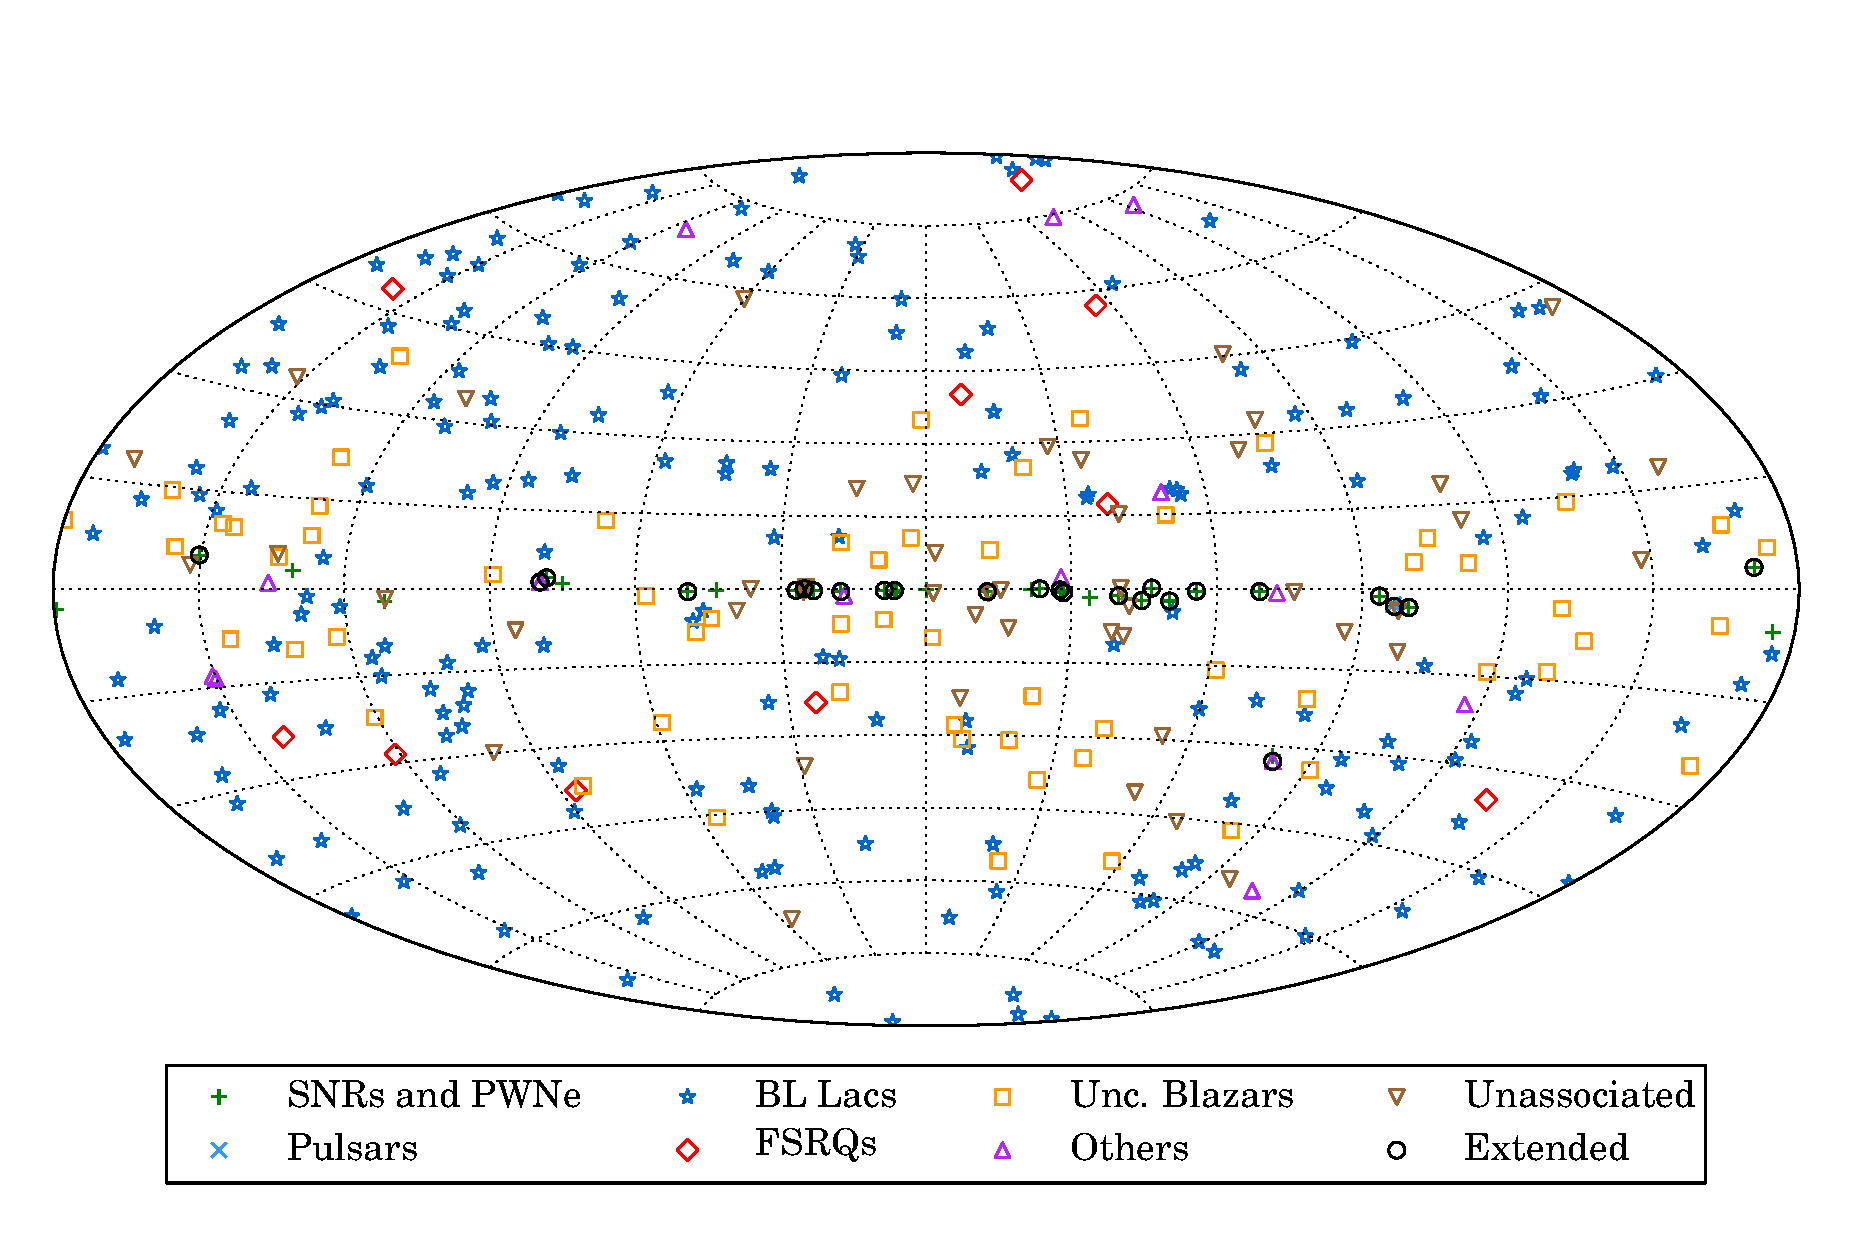
\includegraphics[width=16cm,trim=0 0 0 0cm]{Figures/all-sky_assoc.eps} 
	\caption{Sky map, in Galactic coordinates and Hammer-Aitoff projection,
		showing the sources in the 2FHL catalog classified by their most likely association. 
		\label{fig:all_sky}}
\end{figure*}

The 2FHL catalog includes 360 sources detected over the whole sky, each with a likelihood test statistic of ${\rm TS}\geq 25$ and number of associated photons, $N_{\rm pred}\geq 3$. 
The source association procedure (detailed in \cite{2FHL}) finds that 75\% of the sources in the catalog (274 sources) are extragalactic\footnote{This includes N~157B, an extragalactic pulsar wind nebula (PWN).}, 11\% (38 sources) are of Galactic nature, and 13\% (48 sources) are unassociated (or associated with a TeV source of unknown nature). The unassociated sources are divided between 23 sources located at $|b|<10^{\circ}$, and 25 sources at $|b|\geq 10^{\circ}$. Therefore the fraction of extragalactic sources in the sample is likely larger than 80\,\%.
{ The number of 2FHL sources that have not been reported in 3FGL is 57, 47 of which have not been previously reported in any \lat{} catalog nor in the TeVCat\footnote{\url{http://tevcat.uchicago.edu/}} catalog of \tev{} detected sources, and are thus new $\gamma$-ray sources.}
%The results of the association procedures are summarized in Table~\ref{tab:class}.
Figure~\ref{fig:all_sky} shows the location of 2FHL sources color-coded according to their source class. \jamie{don't include assoc table since I didnt' do that work or include because it summarizes what ws found? }

%%%%%%%%%%%%%%%%%%%%%%%%%%%%%%%%%%%%%%%%%%%%%%%%%%%%%%%%%%%%%%%%
%
%         General Results
%
%%%%%%%%%%%%%%%%%%%%%%%%%%%%%%%%%%%%%%%%%%%%%%%%%%%%%%%%%%%%%%%%
\subsection{General Characteristics of 2FHL Sources}\label{2fhl:General}

The 2FHL sources have $>$ 50\,GeV fluxes ranging from
$\sim$$8\times 10^{-12}$~ph~cm$^{-2}$~s$^{-1}$ to $\sim$$1.3\times 10^{-9}$~ph~cm$^{-2}$~s$^{-1}$
with a median flux of  $2.0\times 10^{-11}$~ph~cm$^{-2}$~s$^{-1}$
and a median spectral index of 2.83. The index uncertainty increases rapidly with the spectral index (\eg the uncertainty is about
$\pm 0.5$ for sources with $\Gamma=2$ whereas it is 
$\pm 2$ for sources with $\Gamma=5$).
Half of the sources are localized to better than
1.7$'$ radius at 68\,\% confidence. 
\jamie{don't include flux vs index stuff}
%Figure~\ref{fig:index_vs_flux} plots the spectral index versus the photon flux for sources associated with extragalactic sources or located at \blot (the extragalactic sample), Galactic sources, and unassociated sources. Figure~\ref{fig:index_vs_flux} shows that there is no visible dependence of the sensitivity (i.e. minimum dethighlighting that the sensitivity for source detection becomes { worse} in the plane of the Galaxy.} 
The distributions of spectral indices and the highest photon energy reported in Figure~\ref{fig:hist_index} show that extragalactic sources tend to have larger photon indices (median of 3.13) than Galactic sources (median of 2.10).   Because of the harder spectra, Galactic sources tend to have higher-energy HEPs than those of extragalactic sources
as shown as well in Figure~\ref{fig:hist_index}.
It is interesting to note that unassociated sources have a median index of 2.22 (2.00 for  sources at \blat and 2.96 for those at \blot), showing that a fraction (see later) of unassociated sources is likely of Galactic origin. 

\jamie{keep this?}Building a spectral energy distribution (SED) represents a powerful way to discriminate or infer the nature of a source. By combining the spectral data from the 3FGL, 1FHL, and 2FHL catalogs, it becomes possible to measure the SEDs
of sources over four decades in energy. Although these catalogs rely on different exposures and  most $\gamma$-ray sources are variable, these data allow us to characterize the high-energy peak of their broadband SEDs. The SEDs of a few notable sources will be shown in the next sections.

%%%%%%%%%%%%%%%%%%%%%%%%%%%%%%%%%%%%%%%%%%%%%%%%%%%%%%%%%%%%%%%%
%
%         Galactic Science
%
%%%%%%%%%%%%%%%%%%%%%%%%%%%%%%%%%%%%%%%%%%%%%%%%%%%%%%%%%%%%%%%%

\subsection{The 2FHL Galactic Source Population}\label{2fhl:GalPop}


The narrow PSF core (about $0.1^{\circ}$) and moderate Galactic diffuse emission (in comparison with the $>100$\,MeV band) allows the LAT to characterize and study well the emission of sources in the plane of our Galaxy above 50\,GeV. Within $|b|<10^{\circ}$, \lat{} has detected 103 sources.
Of those, 38 sources are associated with Galactic sources, 42 with blazars, 14 are unassociated and 9 are associated with other $\gamma$-ray sources
whose origin is not known (see below).
Figure~\ref{fig:gp1} shows cut-outs of the Galactic plane with all detected sources labeled.

\begin{figure*}[!ht]
	\begin{centering}
		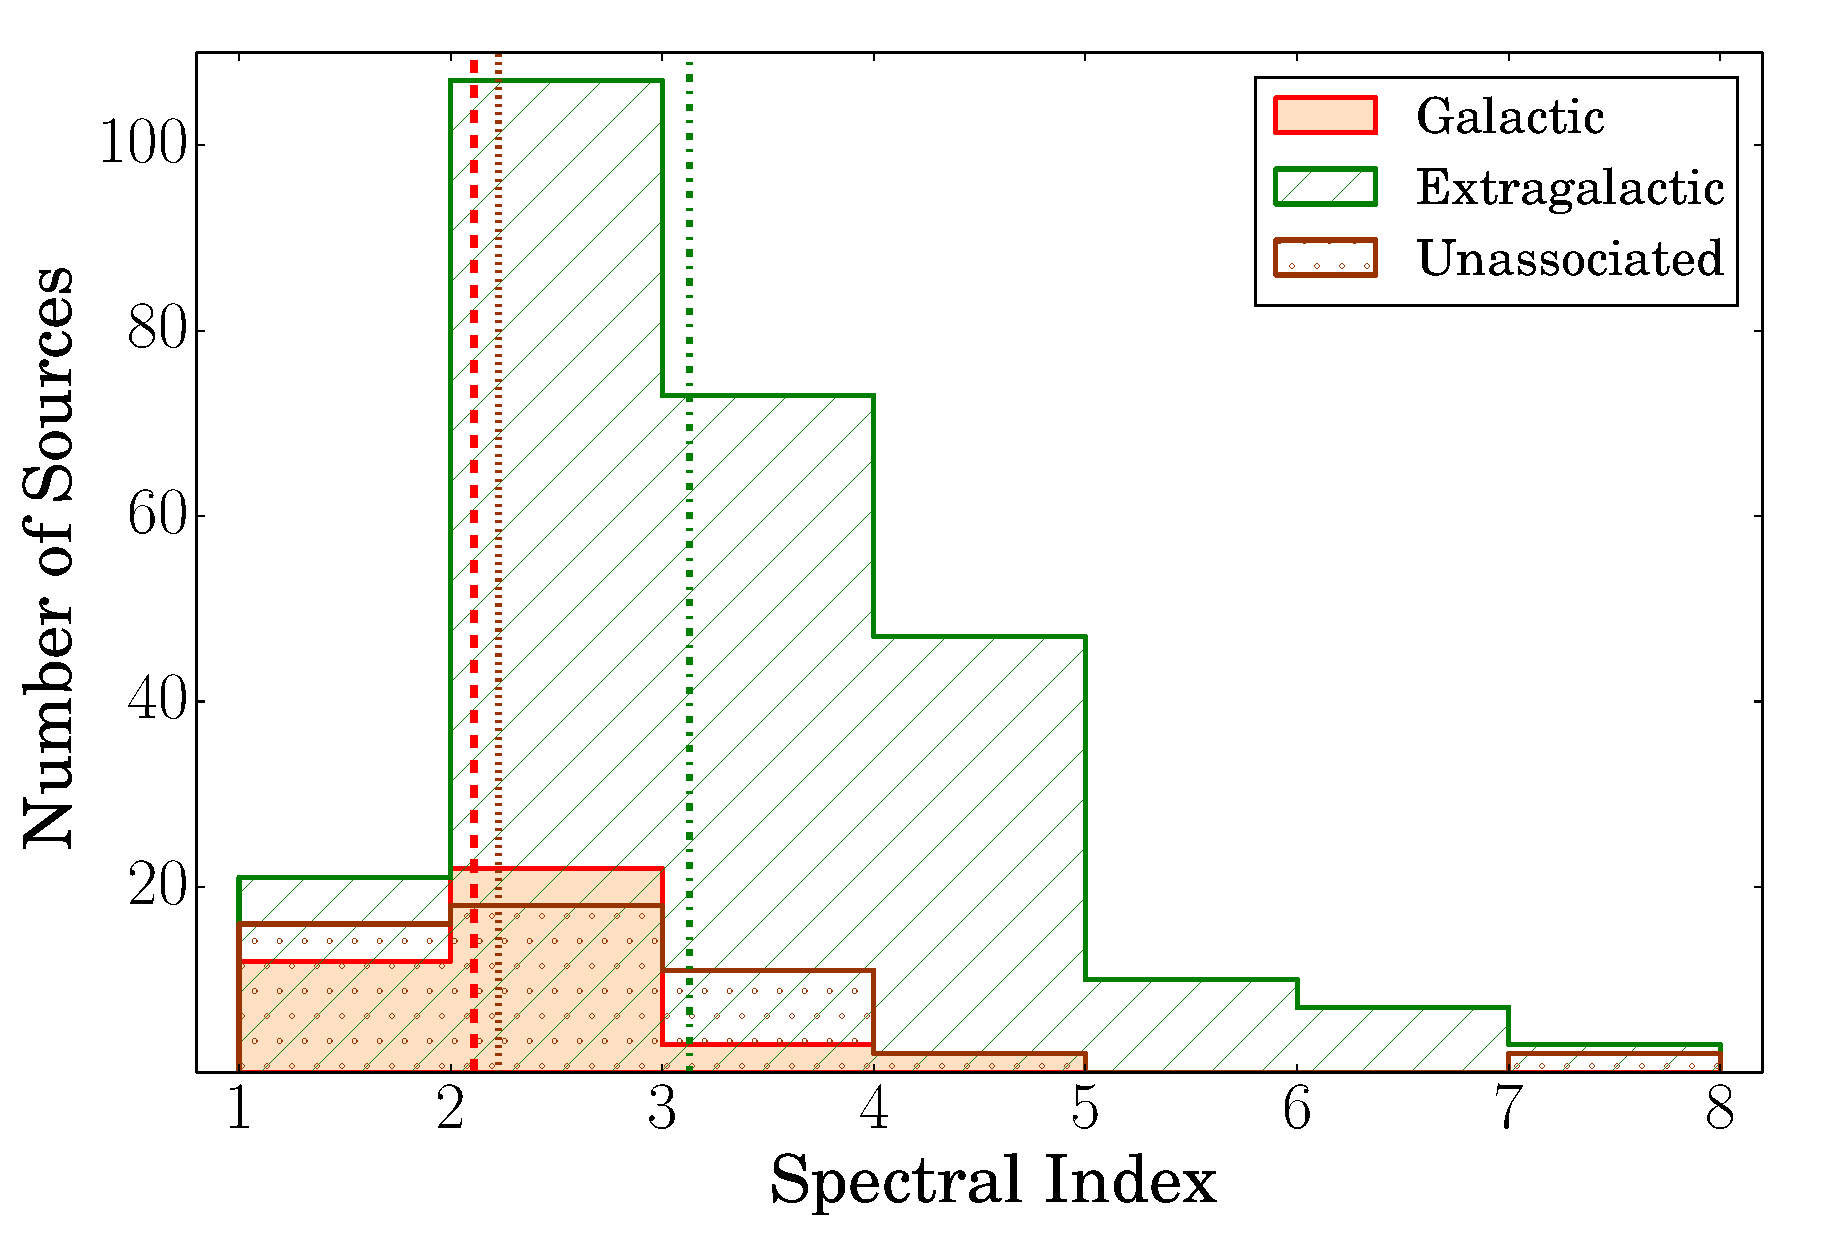
\includegraphics[width=0.9\columnwidth]{Figures/hist_index-new.eps}
		 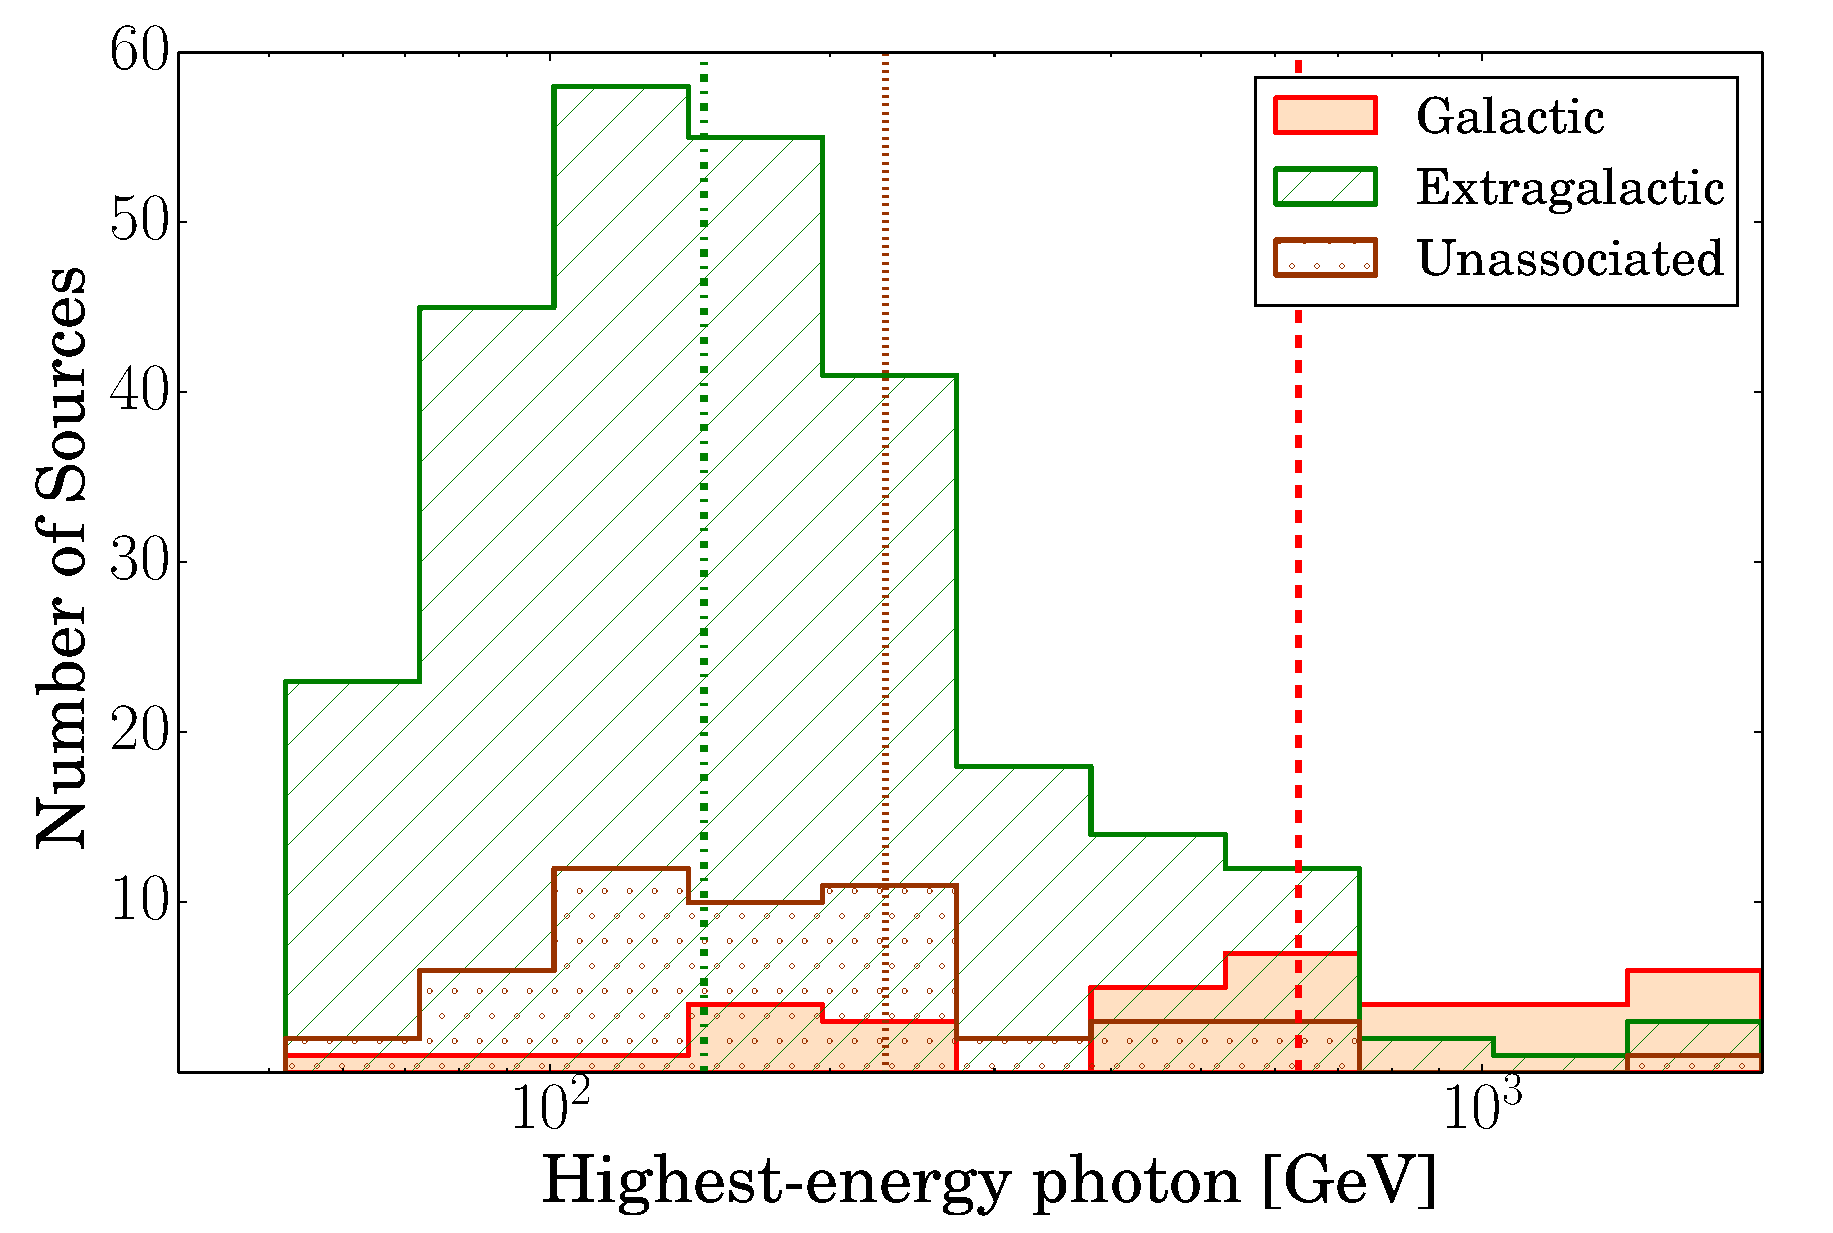
\includegraphics[width=0.9\columnwidth]{Figures/hist_hep-new.eps} 
		\caption{Distribution of the spectral indices ({\it top panel}) and highest photon energy ({\it bottom panel}) of the Galactic sources (orange), extragalactic sources (green slash), and unassociated sources (brown dotted). The medians of the distributions are plotted with dashed, dash-dotted, and dotted vertical lines, respectively. Both plots show that a distinct population of hard-spectrum sources is of Galactic origin.
			\label{fig:hist_index}}
	\end{centering}
\end{figure*}

Among the 38 Galactic sources, 16 are spatially coincident with SNRs, 13 are coincident with PWNe, 4 are associated with PWN/SNR complexes
and the other 5 sources are X-ray binaries (3), one pulsar (PSR~J0835$-$4510)
and the Cygnus Cocoon.
It is clear that the majority of Galactic sources detected above 50\,GeV
are associated with objects at the final stage of stellar evolution.

\begin{figure*}[!ht]
	\begin{center}
		\begin{tabular}{ll}
			% original scale=0.4
			        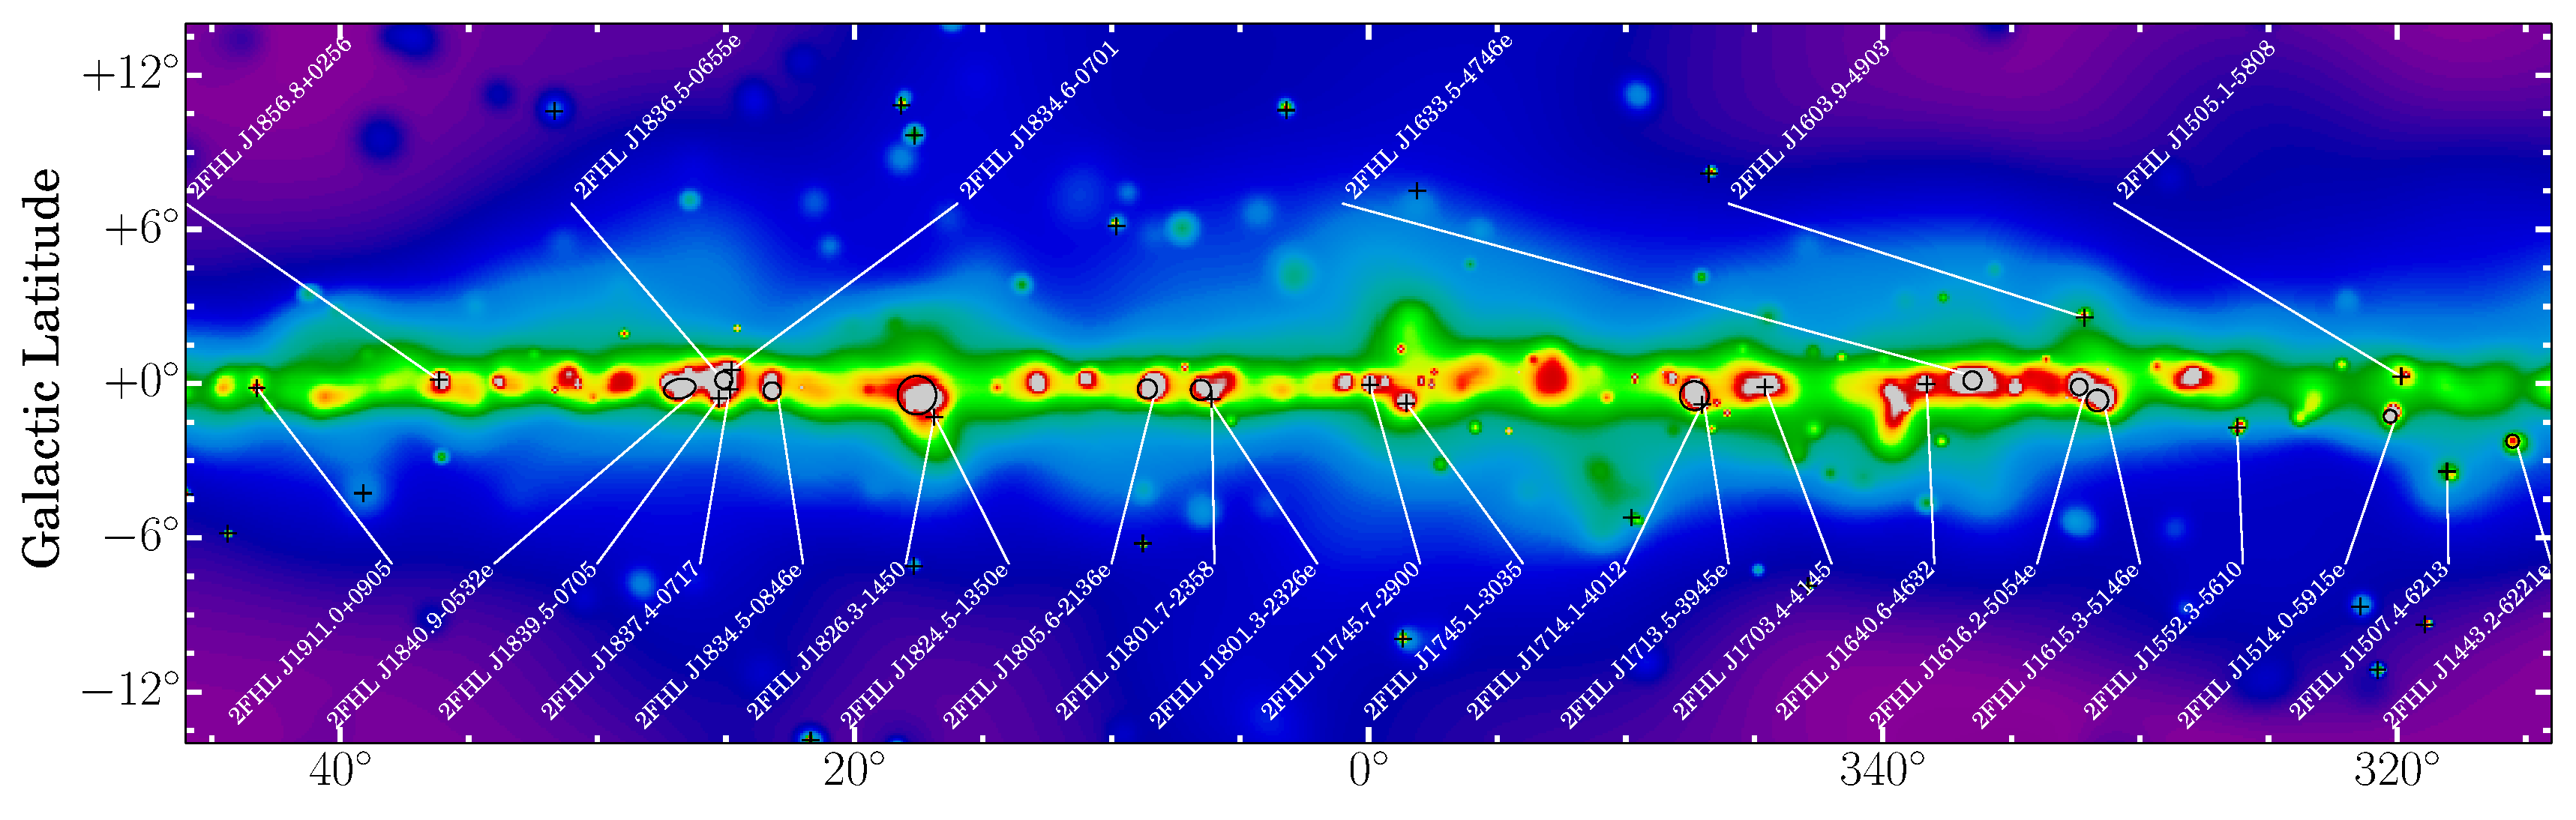
\includegraphics[angle=90,scale=.3]{Figures/Galactic_plane_CAR_1of4_sqrt_spectral_2FHL.eps}&
			        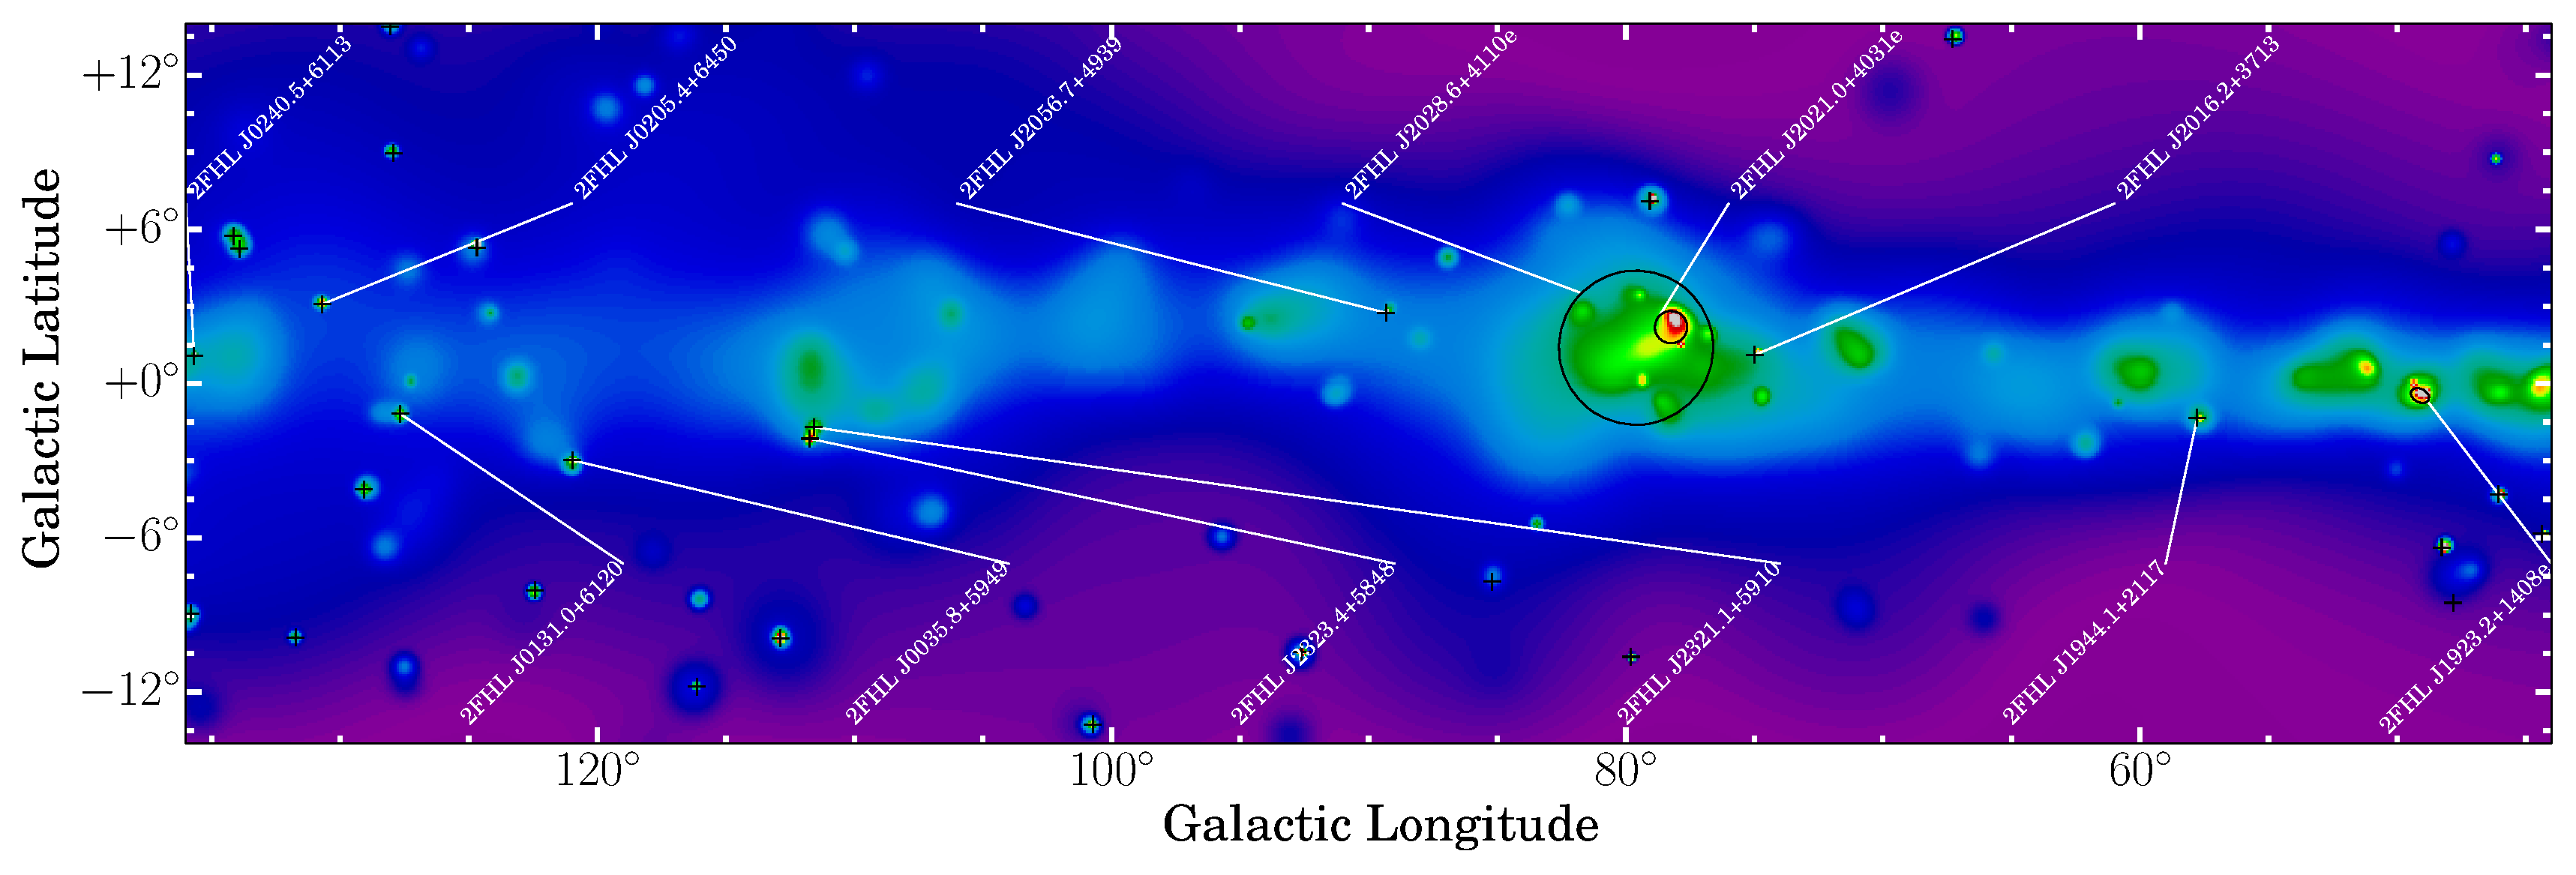
\includegraphics[angle=90,scale=.3]{Figures/Galactic_plane_CAR_2of4_sqrt_spectral_2FHL.eps}\\
			%\includegraphics[angle=90,scale=.3]{f5a.eps}&
			%\includegraphics[angle=90,scale=.3]{f5b.eps}\\
			
			
		\end{tabular}
	\end{center}
	\caption{Adaptively smoothed count map showing the whole Galactic plane $0^{\circ}\leq l\leq 360^{\circ}$ at Galactic latitudes $-14^{\circ} \leq b\leq 14^{\circ}$ divided in four  panels. The panels are centered at $l=0^{\circ}$, $90^{\circ}$, $180^{\circ}$ and $270^{\circ}$, respectively. Detected point sources are marked with a cross whereas extended sources are indicated with  their extensions. Only sources located at $-4^{\circ} \leq b\leq 4^{\circ}$ are explicitly named, plus the Crab Nebula.
		\label{fig:gp1}}
\end{figure*}


\begin{figure*}[!ht]
	\begin{center}
		\begin{tabular}{ll}
			        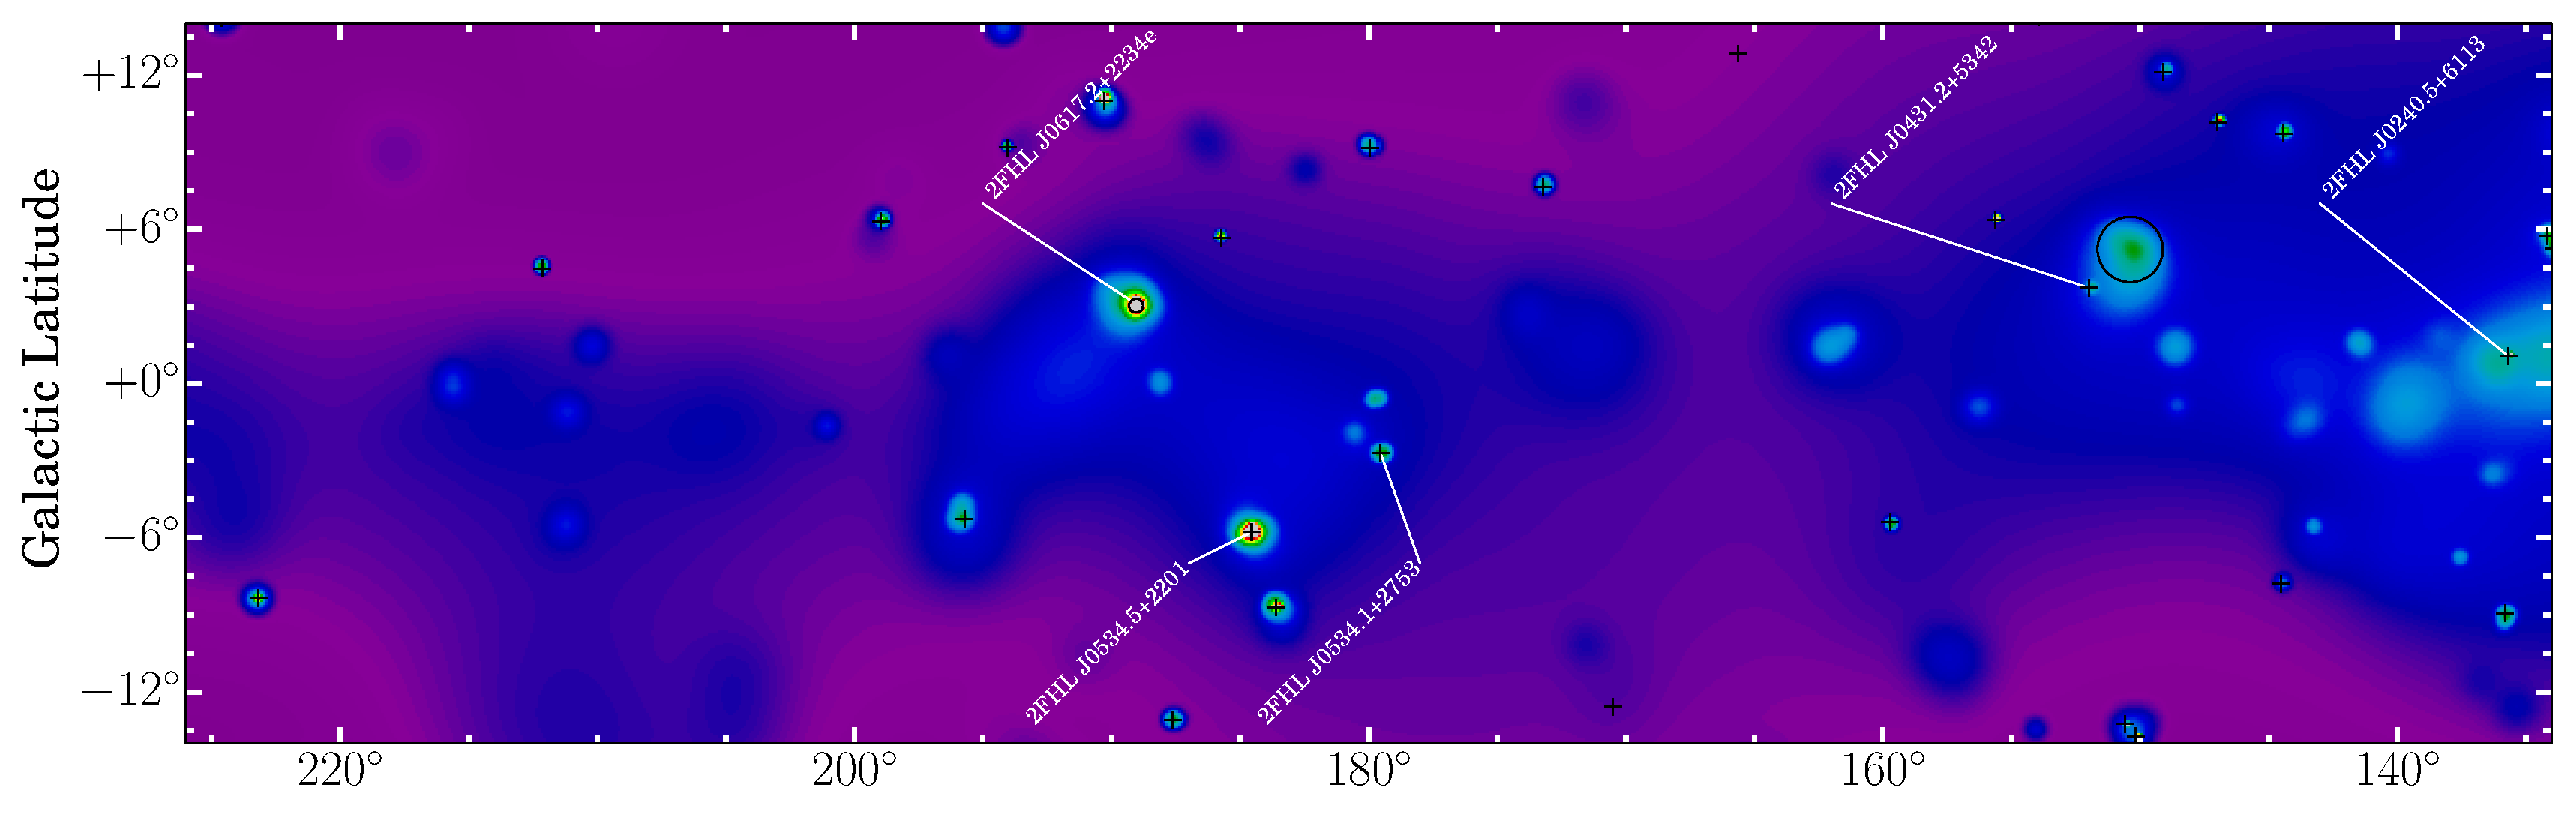
\includegraphics[angle=90,scale=.3]{Figures/Galactic_plane_CAR_3of4_sqrt_spectral_2FHL.eps}&
			        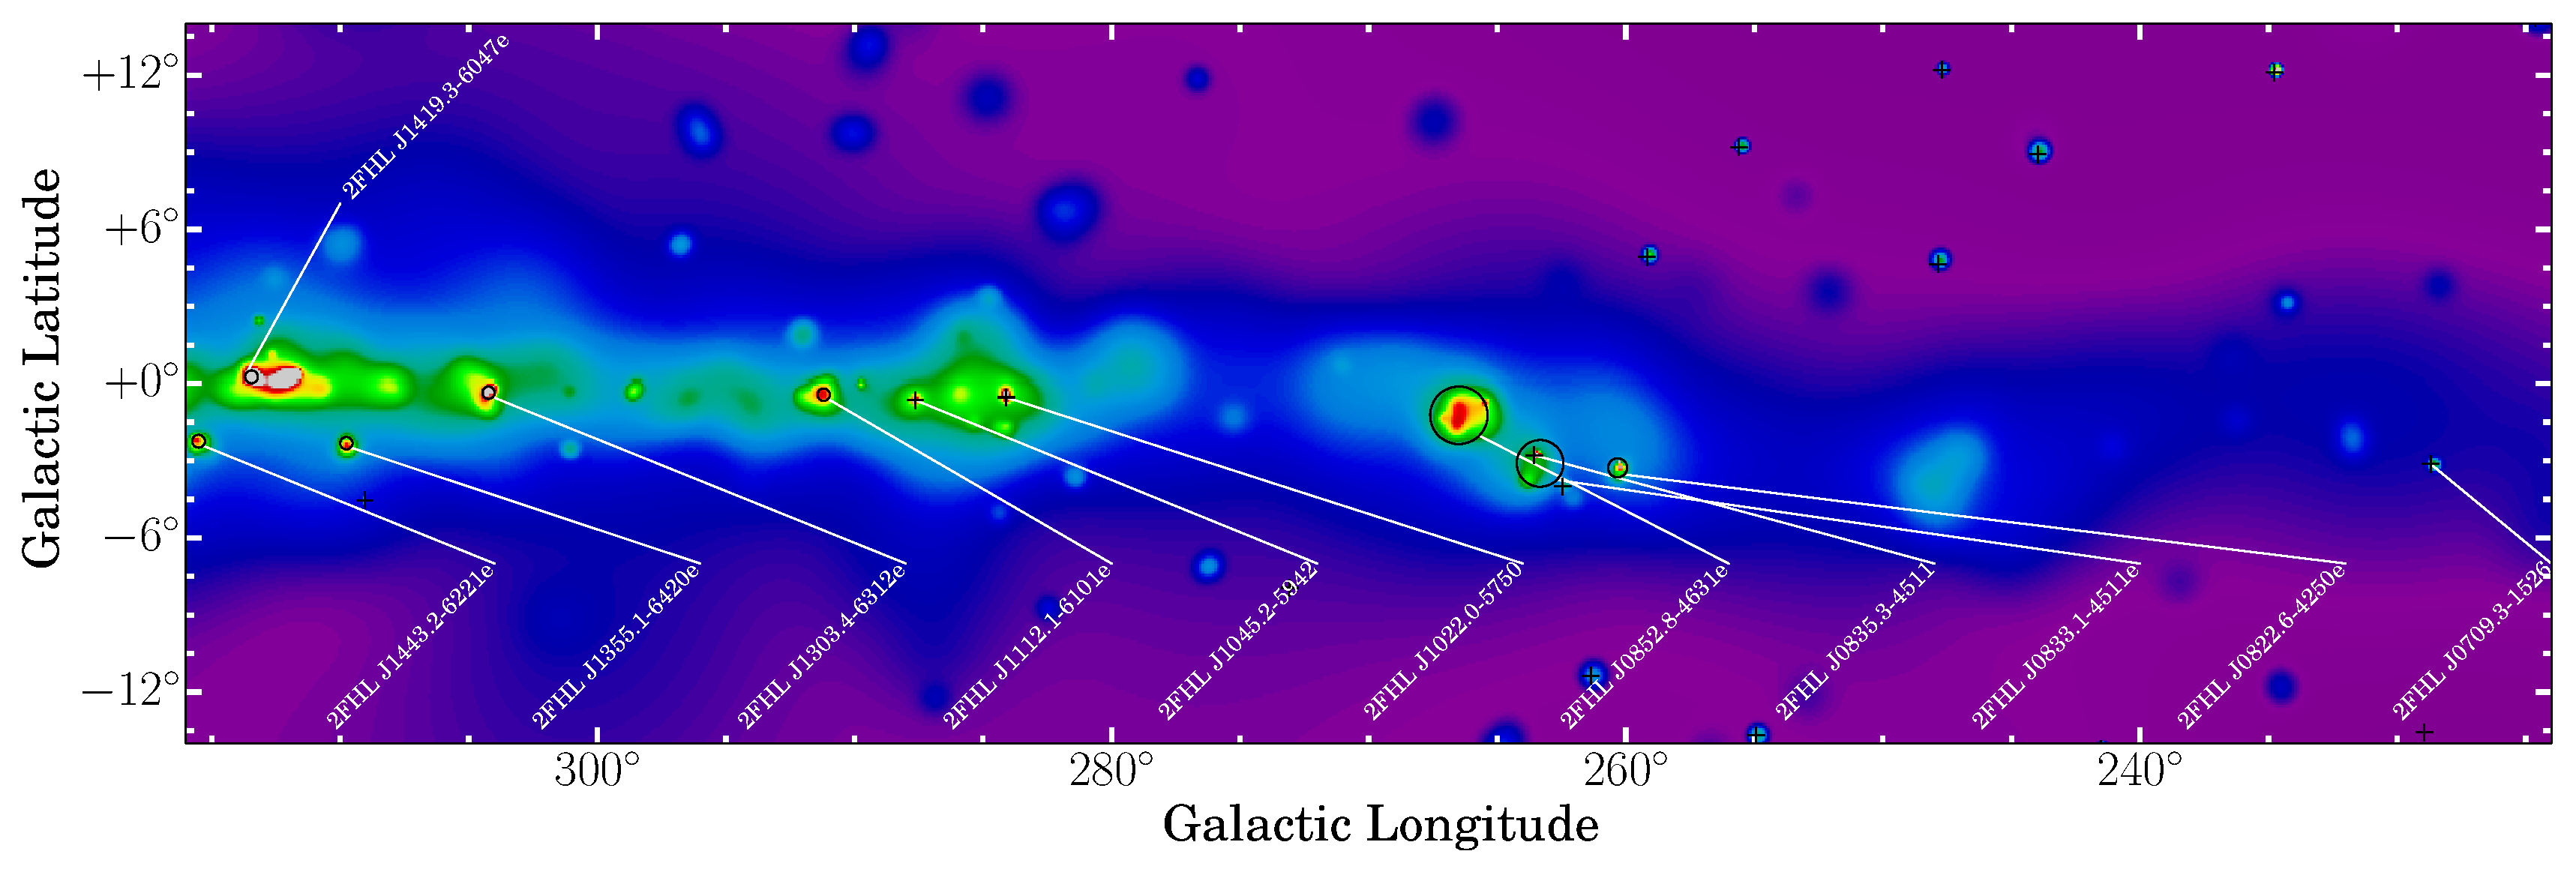
\includegraphics[angle=90,scale=.3]{Figures/Galactic_plane_CAR_4of4_sqrt_spectral_2FHL.eps}\\
			%\includegraphics[angle=90,scale=.3]{f5c.eps}&
			%\includegraphics[angle=90,scale=.3]{f5d.eps}\\
			
		\end{tabular}
	\end{center}
	\begin{flushleft}
		{Fig.~\ref{fig:gp1}.}---  continued
	\end{flushleft}
\end{figure*}

Galactic sources display on average hard spectra, which is a sign
of efficient particle acceleration. Roughly 55\% of all Galactic
sources have a spectral index lower than 2.2. For comparison, only 14\% of the { 2FHL} blazars
display such hard spectra. %With the exception of Eta Carinae (2FHL J1045.2-5942), all hard Galactic sources belong to either the PWN class (12 sources) or the SNR class (8 sources).
A sizable fraction (approximately 25\%, 
see Figure~\ref{fig:hist_index}, upper panel)
of Galactic sources has a photon
index harder than 2, implying a high-energy SED peak in the TeV band.
Indeed, as the lower panel of Figure~\ref{fig:hist_index} shows,
\lat{} detects emission from many Galactic sources well beyond 500\,GeV.
%All these sources belong to either the PWN or SNR classes.
All PWNe detected by {\it Fermi} are found to be powered by young
and energetic pulsars \citep[age $\lesssim 30$\,kyr,][]{Acero13}.
While it is common for PWNe to show hard spectra, this is less
so for SNRs whose majority (about 85\,\%) display softer spectra
\citep{hewittSNRcat13}. Hard-spectrum SNRs are typically young or 
mid-aged ($\lesssim$3--5\,kyr)
and might be difficult to find in radio surveys. Thus, Galactic surveys
at above 50\,GeV have the capability to detect new SNRs that
might have been previously missed.
Such an example is represented by the extended source 
2FHL J0431.2+5553e which is spatially coincident with a 
new SNR (SNR G150.3+4.5) recently reported by \cite{Gao14}.

Of the 14 sources at $|b|<10^{\circ}$ that do not have an
association, 7 have power-law indices harder than 2
which renders them  likely Galactic objects.
It is interesting to note that { 6 of these 7 objects} are offset from the plane of the Galaxy  by more than $4^{\circ}$. This is in marked contrast with the 
associated portion of the sample where only the Crab Nebula and the
newly discovered SNR G150.3+4.5 (out of 34 SNR/PWN systems) have such
a large offset. Thus it seems unlikely that all these unassociated sources
are SNR/PWN systems.

%%%%%%%%%%%%%%%%%%%%%%%%%%%%%%%%%%%%%%%%%%%%%%%%%%%%%%%%%%
%
% H E S S 
%
%%%%%%%%%%%%%%%%%%%%%%%%%%%%%%%%%%%%%%%%%%%%%%%%%%%%%%%%%%%

\subsection{Comparison with the H.E.S.S. Galactic Plane Survey}\label{2fhl:HESS}
The H.E.S.S array, with a field of view of about 5$^{\circ}$ and an angular resolution of approximately 0.12$^\circ$, has invested 2800\,hrs of exposure to survey  part\footnote{The H.E.S.S. Galactic plane survey extends between 283$^{\circ}<l<$59$^{\circ}$ and Galactic latitudes of $|b|<3.5^{\circ}$.} 
of the Galactic plane, reaching an average sensitivity of 2\,\% of the Crab Nebula flux (i.e. 4.5$\times10^{-13}$\,ph~cm$^{-2}$~s$^{-1}$) at $\geq$1\,TeV \citep{aharonian06_gps,carrigan2013}. Considering that the Crab Nebula spectrum is harder
in the 2FHL band than in the $>$1\,TeV band, we estimate that the average sensitivity of 2FHL in the same region of the H.E.S.S. survey is $\sim$3--4\,\% of the { 50\,GeV--2\,TeV Crab Nebula flux.} The slightly better sensitivity 
allows H.E.S.S. to detect 69 sources (as reported in the TeVCat), while
the LAT finds 36 objects in the same area. However, the comparable sensitivities of the two surveys allow the study of the  properties of the high-energy Galactic population.
%%%% USE following to convert the 2% >1TeV Crab nebula flux to
%%%%     2FHL flux
%%%%  4.5e-13*(pow(2.,-1.3)-pow(50./1000.,-1.3))/(pow(100.,-1.3)-pow(1.,-1.3))
%%%%
%%%%  The HESS Crab has an index of 2.3
%%%%  The Fermi Crab has index of 2.13 and flux 1.31e-9 ph/cm2/s
In the 2FHL catalog there is almost an equal number of SNRs and PWNe
in contrast to what is found in the  H.E.S.S. survey where the ratio
of PWNe to SNRs is 1.5 to 1. This might be because
the hardest PWNe and softest SNRs { are difficult to detect} respectively
in the $>$50\,GeV and $>$1\,TeV bands.


Of the 36 2FHL sources that fall within the footprint of 
the H.E.S.S. survey, 23 have already been detected
at TeV energies and are associated with known counterparts,
while 7 are undetected. The remaining 6 objects
(2FHL~J1022.0$-$5750, 2FHL~J1505.1$-$5808,  2FHL~J1507.4$-$6213, 2FHL~J1703.4$-$4145, 2FHL~J1745.1$-$3035 and  2FHL~J1856.8+0256)
are spatially coincident with TeV sources whose origin is not known.
All of them have hard spectral indices ($\Gamma<$2.2), but
it is interesting to note that 4 of them 
(2FHL~J1022.0$-$5750, 2FHL~J1505.1$-$5808, 2FHL~J1703.4$-$4145, and 2FHL~J1745.1$-$3035)
have $\Gamma<1.7$ (see also Figure~\ref{fig:gal_sed}).

We find that 2FHL~J1022.0$-$5750 is spatially compatible with
{ HESS~J1023$-$575, an extended TeV source \citep{westerlund2_hess11},
	whose emission might be due to a PWN powered by PSR~J1023$-$5746 \citep{Acero13}. }
%Westerlund 2 (TeV~J1023$-$5747), a massive star cluster already detected as an extended source at TeV energies \citep{westerlund2_hess11}.
2FHL~J1505.1$-$5808 is spatially coincident with the unidentified
object HESS~J1503$-$582, which has a size of 0.26$^{\circ}$
{ and a flux above 1\,TeV \citep{renaud08} 
	compatible with the extrapolation of the 2FHL J1505.1$-$5808 spectrum.}
Its spectrum, reminiscent of that of a PWN 
\citep[\eg, HESS~J1825$-$137,][]{grondin2011} is reported in Figure~\ref{fig:gal_sed}.


2FHL~J1507.4$-$6213 is spatially coincident with HESS~J1507$-$622, an extended source with a radius of 0.15$^{\circ}$ located  3.5$^{\circ}$ from the plane \citep{acero11}. The analysis of multiwavelength data showed that it is not possible to discriminate between a hadronic and leptonic origin of the emission, but that the latter scenario, if the emission is powered by a PWN, would require a pulsar generated in the explosion of a hyper-velocity star in order to reach the required distance from the plane \citep{domainko2012}.



The sources 2FHL~J1703.4$-$4145 and 2FHL~J1745.1$-$3035 are the hardest sources ($\Gamma<1.3$) among the six objects.
2FHL~J1703.4$-$4145 is spatially coincident with the bright radio emission
observed from the western side of the shell of SNR G344.7$-$001,
a nearby mid-aged  shell-type (age $\sim3000$\,yr and 8$'$ diameter) SNR \citep{giacani2011}. Both the 2FHL source and the SNR are spatially coincident
with the larger, elongated and unidentified HESS~J1702$-$420 \citep{aharonian08}.
It thus seems likely that  SNR G344.7$-$001 is the  counterpart
of  2FHL J1703.4$-$4145 and perhaps also of HESS~J1702$-$420.
The combined {\it Fermi}-H.E.S.S. spectrum of this source is reported in Figure~\ref{fig:gal_sed}.



2FHL~J1745.1$-$3035 is found to be spatially coincident with 
the extended source HESS~J1745$-$303, which may be comprised of
up to three different sources \citep{aharonian2008_j1745}. Indeed, the position of
2FHL~J1745.1$-$3035 is compatible  with the 'C' emission
region \citep[the second brightest region in the complex,][]{aharonian2008_j1745}.
However, the nature of this source is more complex, because
the 2FHL source is marginally brighter at 1\,TeV than the entire H.E.S.S. region and has also a harder spectrum (spectral index of 1.25$\pm0.38$ in 2FHL 
versus $2.17\pm 0.11$ as measured by H.E.S.S.).

Finally, 2FHL~J1856.8+0256 is coincident with HESS~J1857+026, an almost radially symmetric extended source  \citep{aharonian08_unid}, whose emission likely originates from a PWN powered by PSR~J1856+0245 \citep{rosseau2012}.



\begin{figure*}[ht]
	\begin{center}
		\begin{tabular}{ll}
			\includegraphics[width=8cm]{Figures/{J0617.2+2234e_SED}.eps} &
			\includegraphics[width=8cm]{Figures/{J1419.3-6047e_SED}.eps}\\
			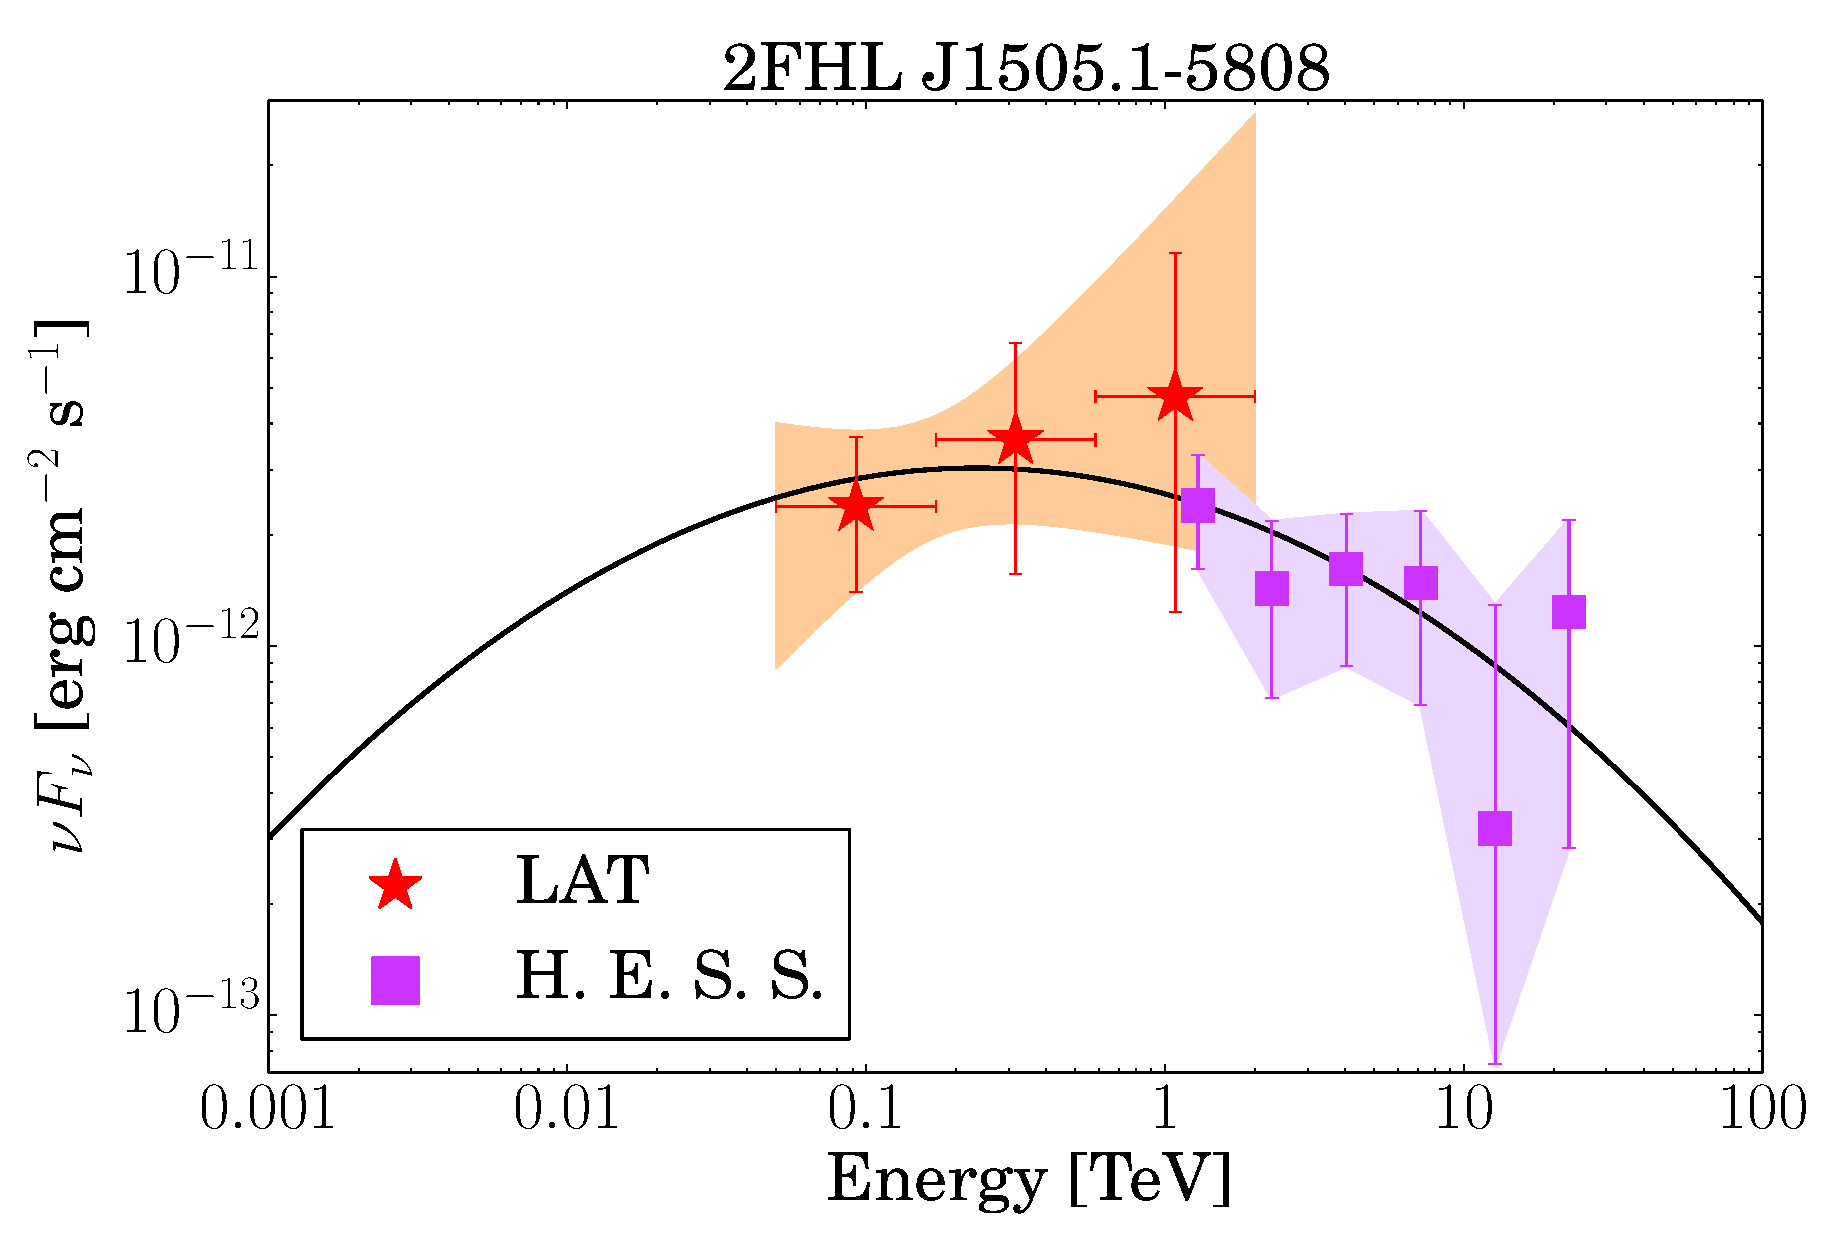
\includegraphics[width=8cm]{Figures/pgw_00682_SED.eps} &
			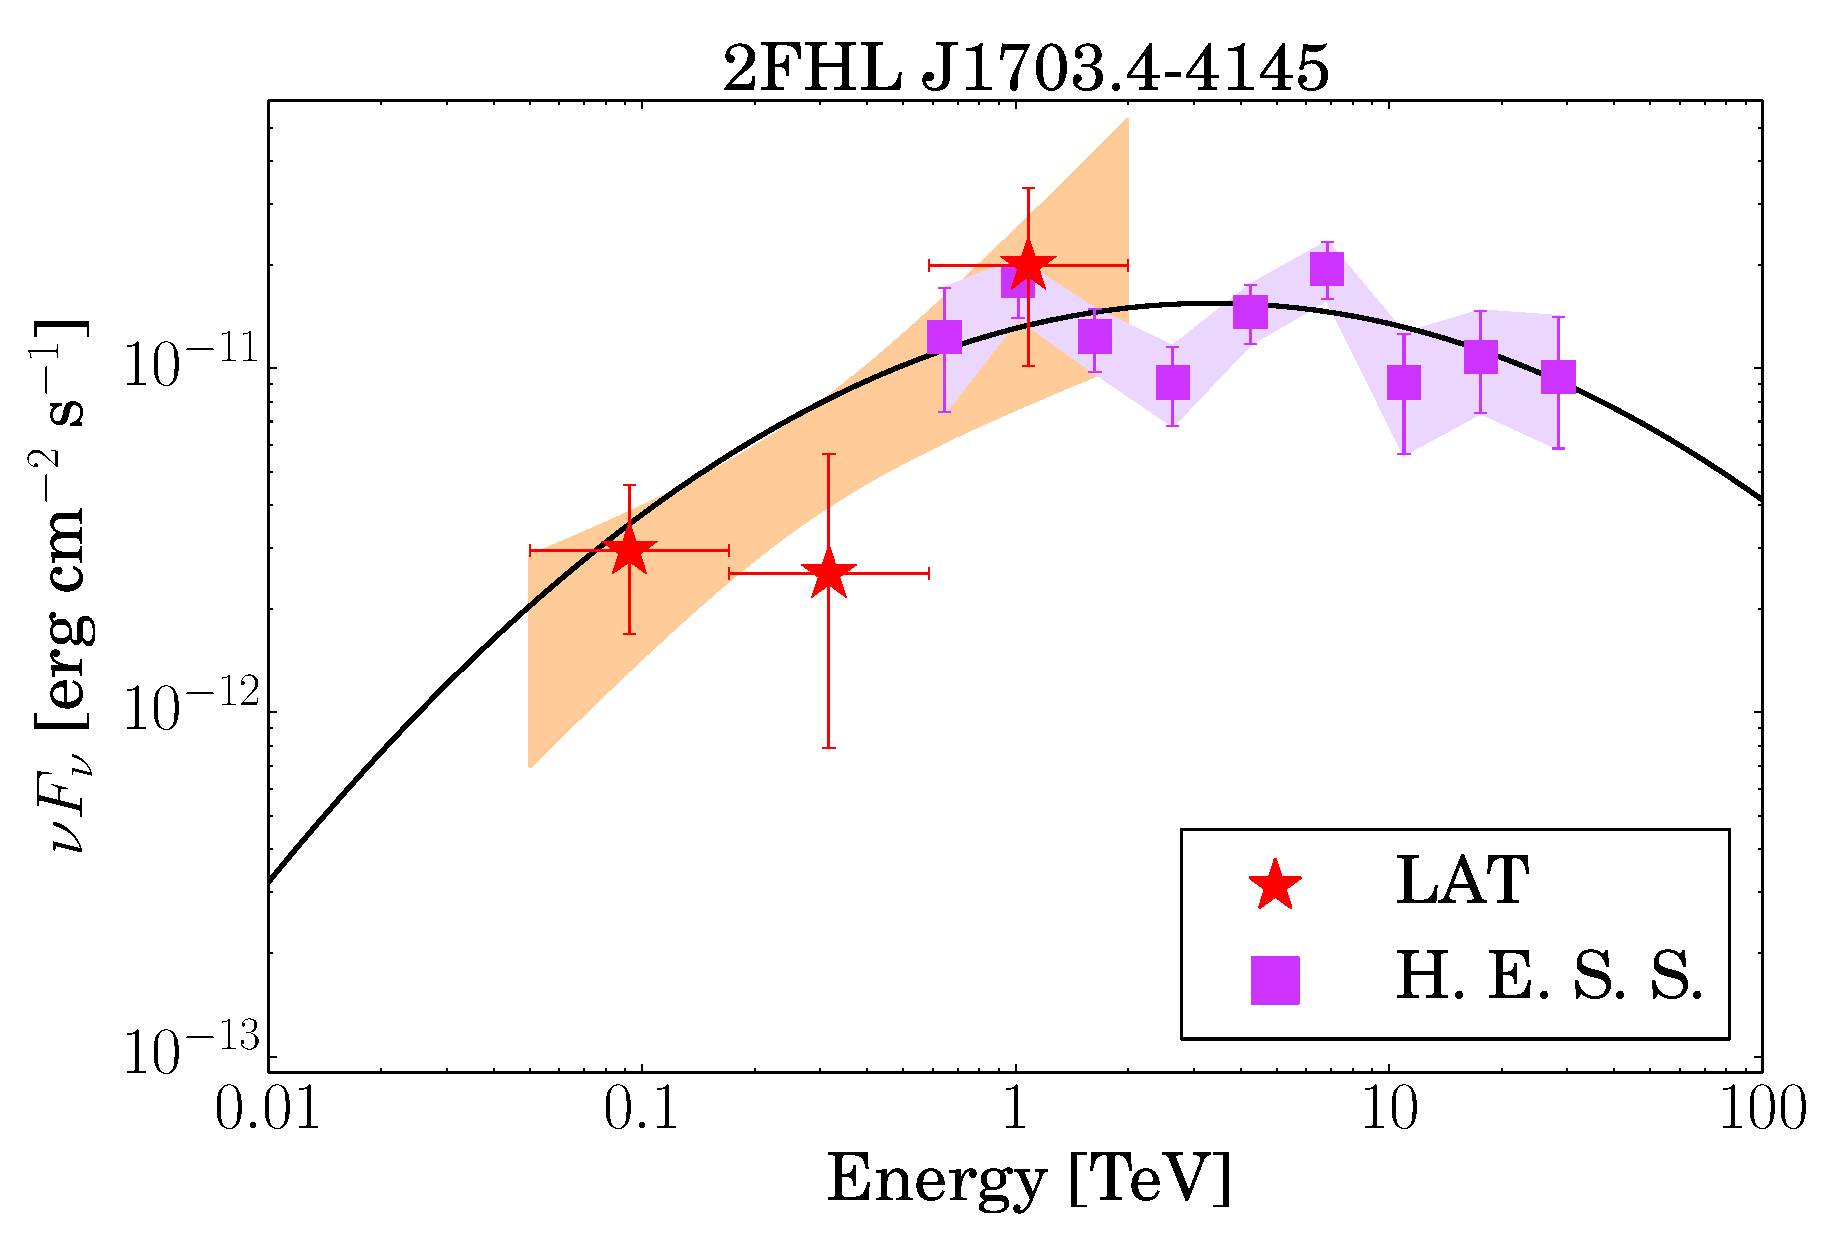
\includegraphics[width=8cm]{Figures/pgw_00110_SED.eps} \\
		\end{tabular}
	\end{center}
	\caption{
		\label{fig:gal_sed}Spectral energy distributions of four Galactic sources constructed by combining data from the 3FGL (green diamonds), 1FHL (blue circles), and 2FHL (red stars). We show the 3FGL extended source SNR IC~443 (\emph{top left}), the new 2FHL extended source PSR~J1420$-$6048 (\emph{top right}), and two ``dark accelerators'' detected by H.E.S.S. at TeV energies \citep[][purple squares]{carrigan2013} without a previous LAT counterpart:  { HESS~J1503$-$582} (\emph{bottom left}) and HESS~J1702$-$420 (\emph{bottom right}).}
\end{figure*}

%%%%%%%%%%%%%%%%%%%%%%%%%%%%%%%%%%%%%%%%%%%%%%%%%%%%%%%%%%%%%%%%%%%
%
%  Extended Source Results
%
%%%%%%%%%%%%%%%%%%%%%%%%%%%%%%%%%%%%%%%%%%%%%%%%%%%%%%%%%%%%%%%

\subsection{\label{2fhl:ESresults}Extended Source Results}


In total, 31 sources are modeled as spatially extended and input into the ML analysis: 25 listed in 3FGL, 5 sources detected in the {\tt pointlike} analysis (described in $\S$ \ref{sec:3FGL_ES}) that were not { detected as extended at the time of} 3FGL, and one, SNR W41, reported  recently by both the H.E.S.S. and LAT teams \citep{HESSLATW41}. Names and properties of the extended sources  are provided in Tables \ref{tab:extended} and \ref{tab:new_extended}. 
Six extended sources, detected in 3FGL, were not detected in 2FHL: the SMC, S~147 ({the point source 2FHL~J0534.1+2753 was detected inside it}), the lobes of Centaurus A (although we detect its core as a point source, 2FHL J1325.6$-$4301), W~44, HB~21 and the Cygnus Loop.

We detect a weak source, 2FHL~J1714.1$-$4012 (TS = 27), just outside the southwestern edge of the 3FGL spatial template used to model the emission from SNR RX J1713.7$-$3946 (2FHL~J1713.5$-$3945e). 2FHL~J1714.1$-$4012 has a hard spectral index $\Gamma = 1.63 \pm 0.38$, that is within errors of the spectral index derived for the SNR, $\Gamma = 2.03 \pm 0.20$. It is unclear whether 2FHL~J1714.1$-$4012 is a distinct source separated from the SNR, or the result of un-modeled residual emission due to an imperfection in the spatial template adopted for the extended source.


2FHL~J1836.5$-$0655e is associated with the PWN HESS J1837$-$069. The 3FGL catalog contains  several point sources in the vicinity of the PWN. We detect three sources in the vicinity, 2FHL~J1834.5$-$0701, 2FHL~J1837.4$-$0717 and 2FHL~J1839.5$-$0705, the first two of which are coincident with 3FGL sources (3FGL J1834.6$-$0659, 3FGL J1837.6$-$0717 respectively). The power-law spectral indices of the three 2FHL point sources and 2FHL J1836.5$-$0655e are all consistent with each other. The concentration of sources around HESS J1837$-$069 combined with the spectral compatibility of the sources is suggestive of a common origin to the $\gamma$-ray emission in this region. However, the surrounding $\gamma$ rays could arise from other sources in the region \citep{Gotthelf08}; further analysis is necessary to determine the nature of the sources in this region. 

A brief description of the five new 2FHL extended sources is given below with residual TS maps for the region surrounding each source shown in Figure \ref{fig:6ES}. Detailed analyses of these new extended sources will be reported in separate papers.


{\bfseries 2FHL~J1443.2$-$6221e} overlaps with the young, radio-detected SNR RCW 86 (G315.4−2.3). RCW 86 is a 42$'$ diameter SNR that lies at a distance of 2.3-2.8 kpc and is likely associated with the first recorded supernova, SN 185 AD \citep{Rosado96,Sollerman03}. With more than 40 months of data and using the {\tt P7SOURCE} dataset, the LAT did not significantly detect the SNR, but upper limits on detection at GeV energies combined with detection of significant extension in the TeV \citep{Aharonian09} were sufficient to strongly favor a leptonic origin for the emission \citep{Lemoine-Goumard12}.

An updated LAT analysis of RCW~86 using 76 months of data, as well as the Pass 8 event-level analysis, resulted in detection of the SNR by the LAT as well as significant extension measurement \citep{Hewitt15}. In this paper, we report the results derived for 2FHL~J1443.2$-$6221e from the {\tt pointlike} analysis described in $\S$ \ref{sec:3FGL_ES}.

{\bfseries 2FHL~J1419.2$-$6048e} is a newly detected extended sources with size
%an extended source from which we detect for the first time with the LAT significant GeV extension, 
${\rm \sigma_{disk} =  0.36 ^{\circ} \pm}$ $0.03 ^{\circ}$, that overlaps two nearby PWN/PSR complexes in the Kookaburra region. In the southwest of Kookaburra, HESS~J1418$-$609 \citep{AharonianKook06} is coincident with both the extended non-thermal X-ray ``Rabbit" PWN \citep[G313.3+0.1,][]{Roberts99}, and the $\gamma$-ray detected pulsar PSR~J1418$-$6058 \citep{AbdoBlindPSR09}. The northeast region, called ``K3", contains HESS~J1420$-$607, coincident with PWN~G313.5+0.3 and PSR J1420$-$6048. \cite{Acero13} detected, with \lat, emission from both HESS~J1418$-$609 (with a soft spectral index, pulsar-like spectrum) and HESS~J1420$-$607 (with a hard power-law index) above 10 GeV, but only HESS J1420$-$607 was significantly detected above 30 GeV. Neither showed significant extension. Our result for the fitted power-law spectral index of 2FHL~J1419.2$-$6048e is in agreement with the previous GeV and TeV results, yet our measured radius is considerably larger than the TeV extension. To compare the extensions of the uniform disk model used for 2FHL~J1419.2$-$6048e in this paper to the Gaussian model of \cite{AharonianKook06}, we defined the radius which contains 68\% of the source's intensity as r$_{68}$, with ${\rm r_{68,Gaussian} = 1.51\sigma}$, and ${\rm r_{68,disk} = 0.82\sigma}$  \citep{Lande12}. We find that ${\rm r_{68} \simeq 0.30^{\circ}}$ for 2FHL~J1419.2$-$6048e, and ${\rm r_{68}} \simeq 0.09^{\circ}$ for HESS~J1420$-$607.

{\bfseries 2FHL J1355.2$-$6430e}, coincident with the VHE source HESS J1356$-$645, is detected as extended (${\rm \sigma_{disk} =  0.57^{\circ} \pm 0.02^{\circ}}$) for the first time by the LAT in this work. The  source HESS J1356$-$645 \citep{Abramowski11} is associated with the pulsar PSR J1357$-$6429, which was determined to be powering a surrounding extended radio and X-ray PWN \citep{Lemoine-Goumard11}. \cite{Acero13} detected faint emission from the nebula, and derived a 99\% c.l. Bayesian upper limit on extension (${\rm \sigma_{Gauss} < 0.39^{\circ}}$) in the absence of significant extension. The fitted spectral index for 2FHL J1355.2$-$6430e is compatible with the GeV and TeV results \citep{Acero13,Abramowski11}, however, the fitted disk extension is larger than that of the TeV detection, with ${\rm r_{68} \simeq 0.47^{\circ}}$ for 2FHL~J1355.2$-$6430e and ${\rm r_{68}}$ $\simeq 0.30^{\circ}$ for HESS~J1356$-$645.

{\bfseries 2FHL J1112.4$-$6059e} is an extended source (${\rm \sigma_{disk} =  0.53^{\circ} \pm 0.03^{\circ}}$) newly detected by the LAT that encircles two 3FGL sources, 3FGL J1111.9$-$6058 and 3FGL J1111.9$-$6038, and has another, 3FGL J1112.0$-$6135, just outside its boundary \citep{3FGL}. The extended source also partially overlaps the massive star forming region NGC 3603. %A detailed LAT analysis of this region is underway and will be presented elsewhere. % MA COMMENTED it. in \jamie{need a ref for Junichiro's work}.

Finally, {\bfseries 2FHL J0431.2+5553e} is a large extended source (${\rm \sigma_{disk} =  1.27^{\circ} \pm 0.04^{\circ}}$), with { a hard spectrum}, that has not been previously detected at $\gamma$-ray energies. It overlaps the recently discovered radio SNR G150.3+4.5 \citep{Gao14}. G150.3+4.5 is a ${\rm 2.5^{\circ}}\times {\rm 3^{\circ}}$ (Galactic coordinates)
% wide (GLON) and ${\rm 3^{\circ}}$ high (GLAT) 
elliptical shell type SNR that has a steep radio synchrotron spectrum ($\alpha = -0.6$), indicative of radio SNRs.% An in depth LAT analysis of this source extending to energy $E>1$~GeV is in preparation. 


\begin{figure*}[ht]
	\begin{center}
		\begin{tabular}{ll}
			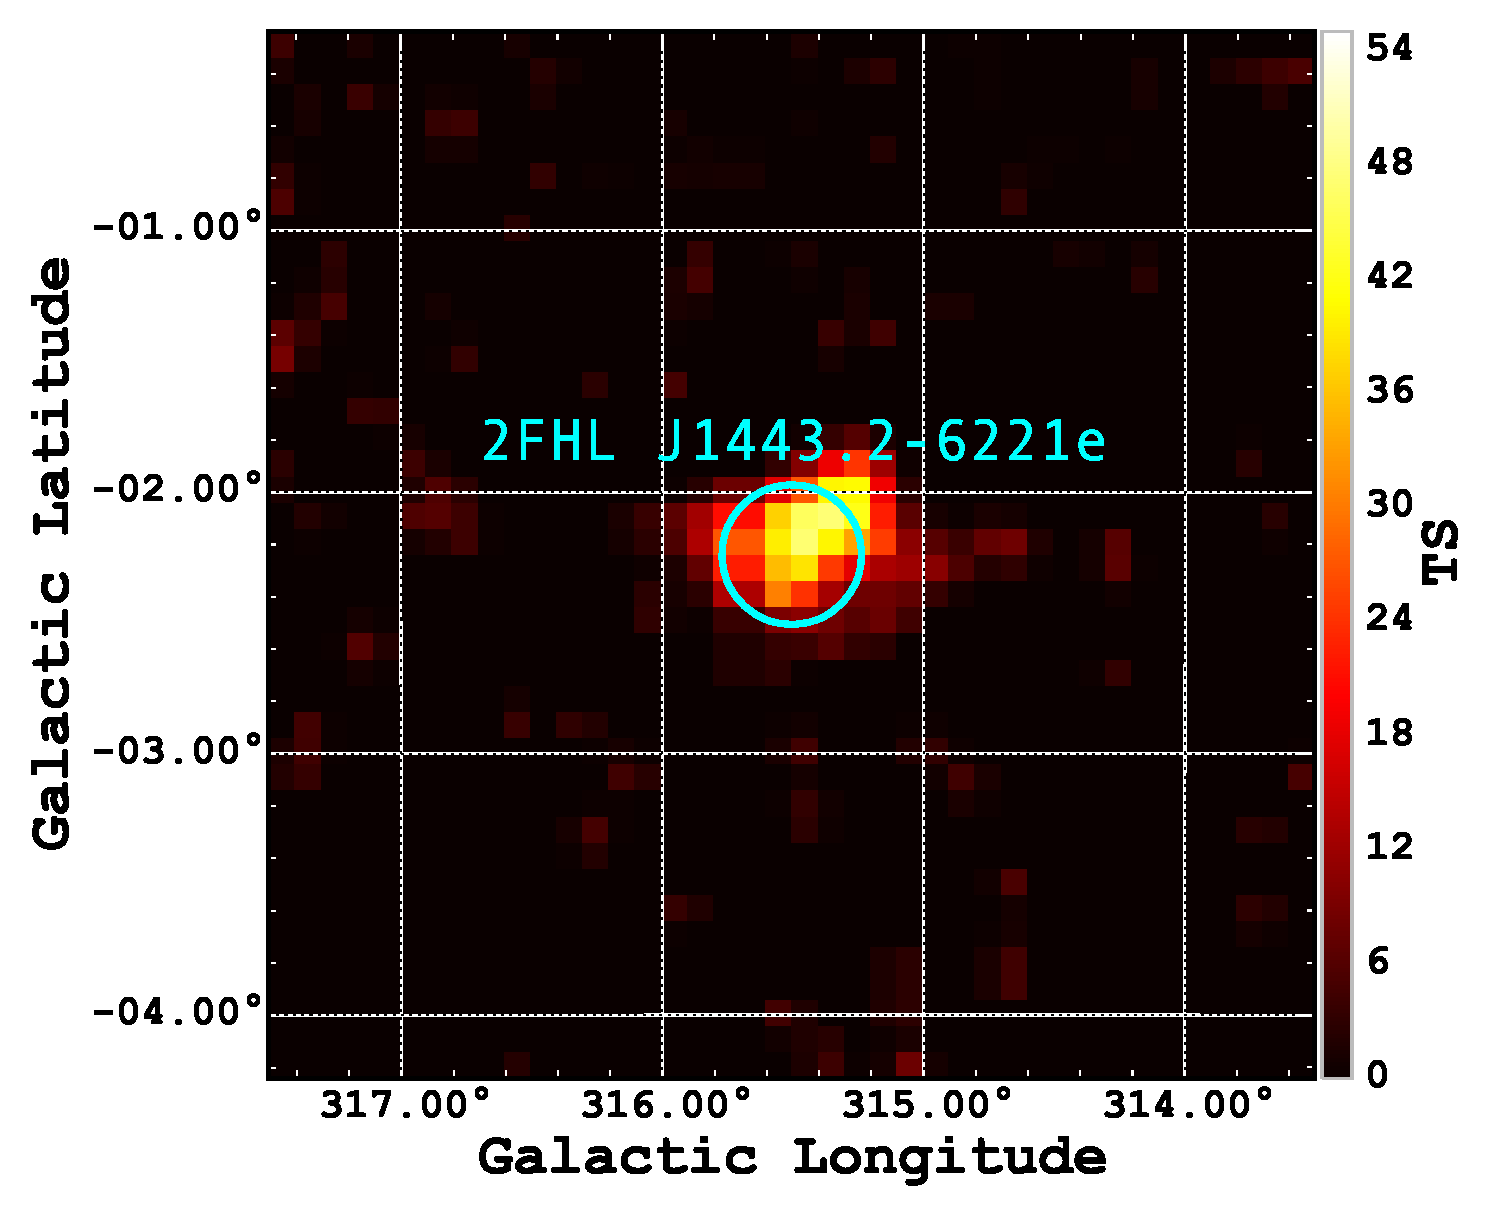
\includegraphics[width=8cm]{Figures/l315_b0_ES_3_residTSmap_2FHL_zoom.eps} &
			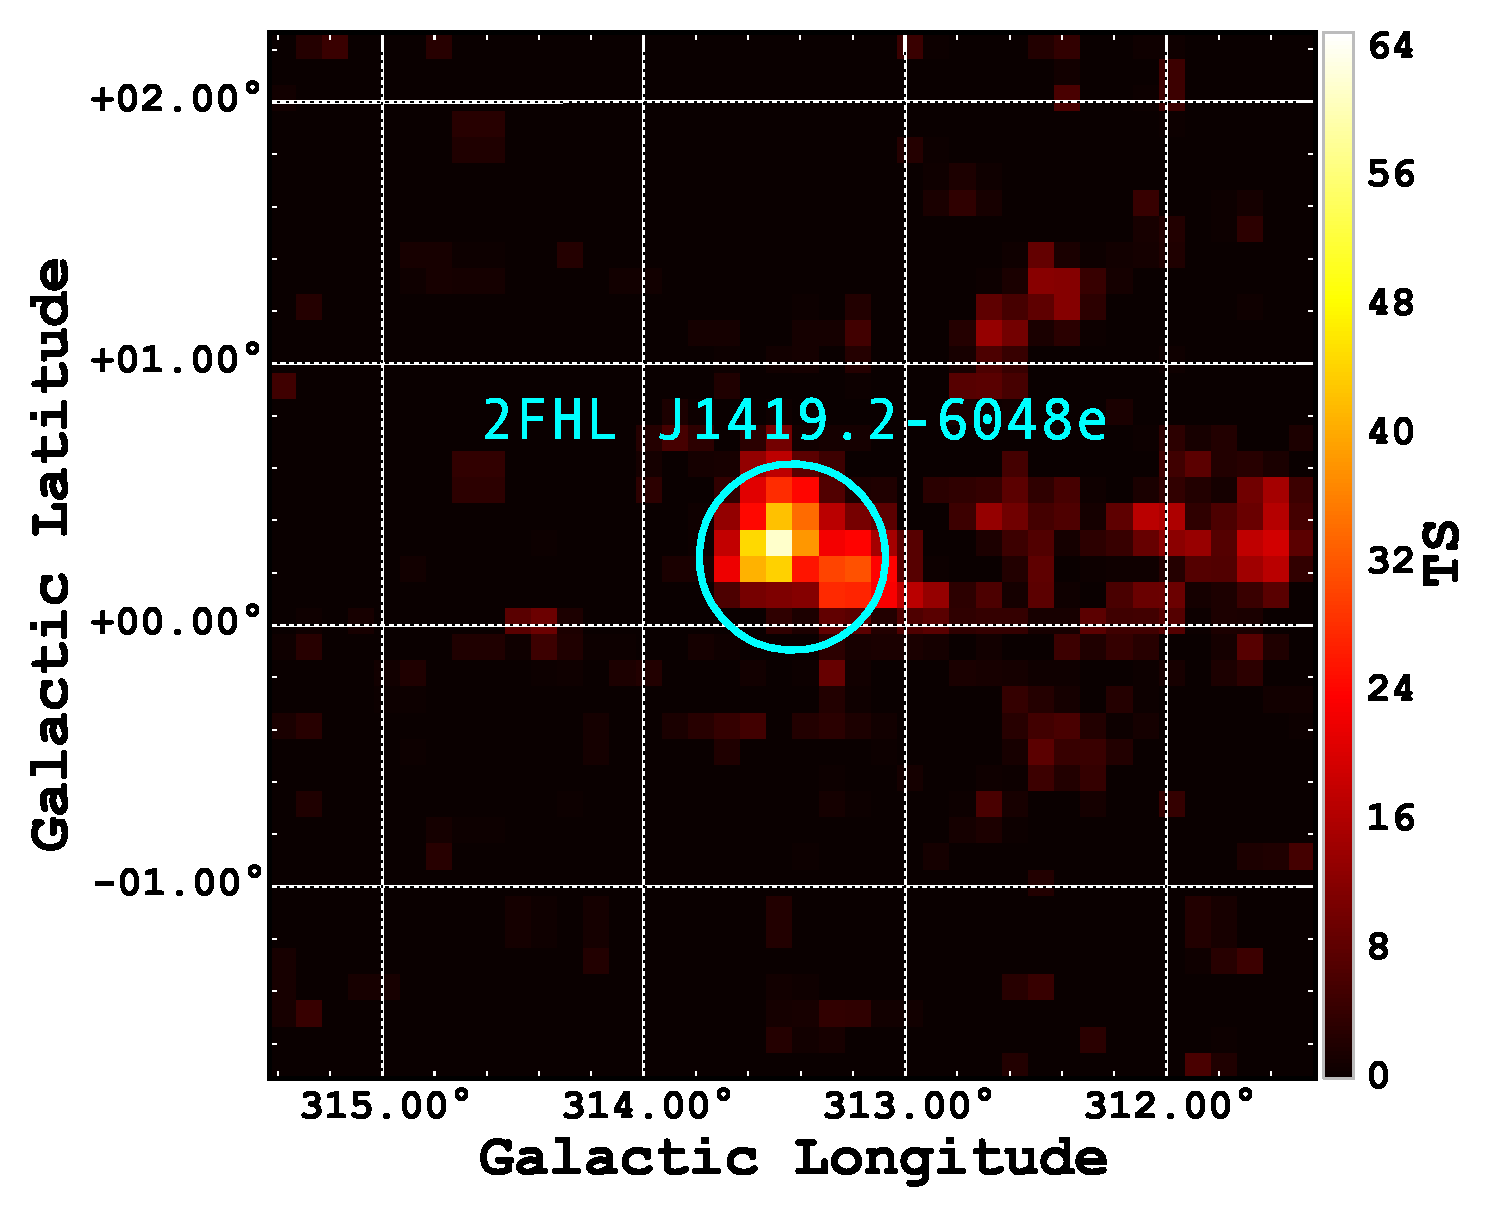
\includegraphics[width=8cm]{Figures/l315_b0_ES_4_residTSmap_2FHL_zoom.eps}\\
			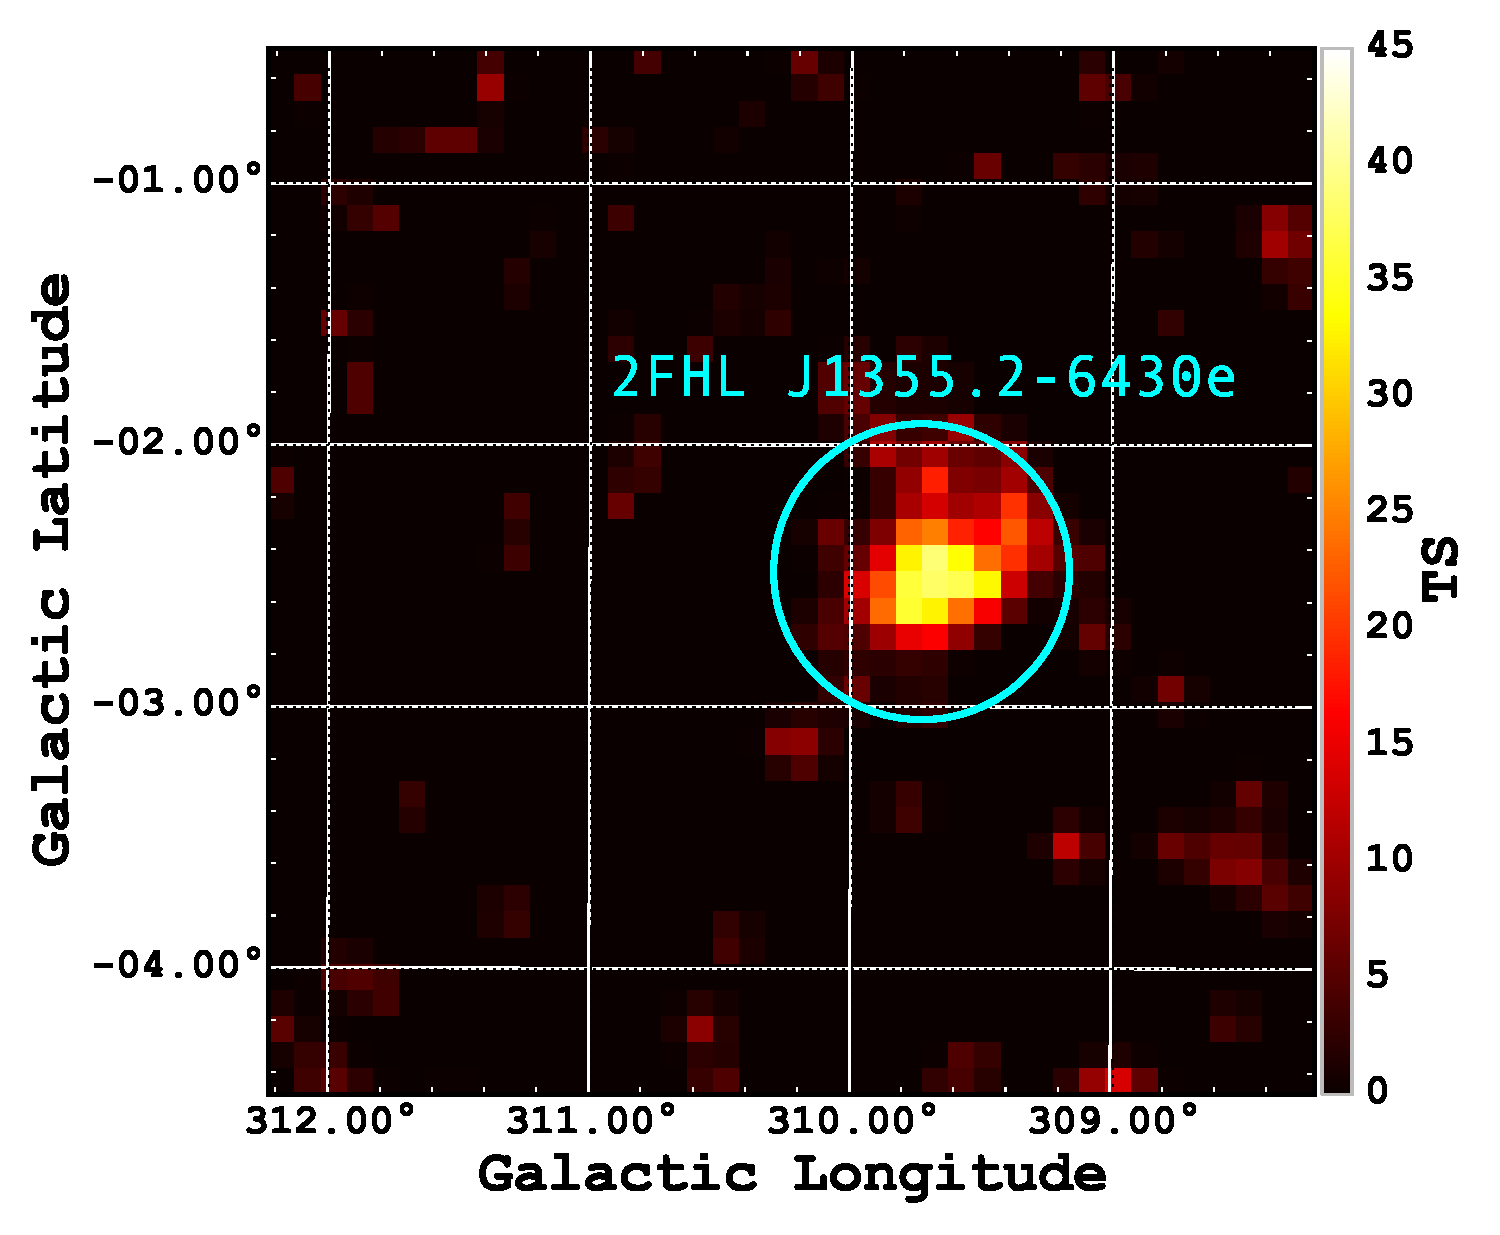
\includegraphics[width=8cm]{Figures/l315_b0_ES_1_residTSmap_2FHL_zoom.eps} &
			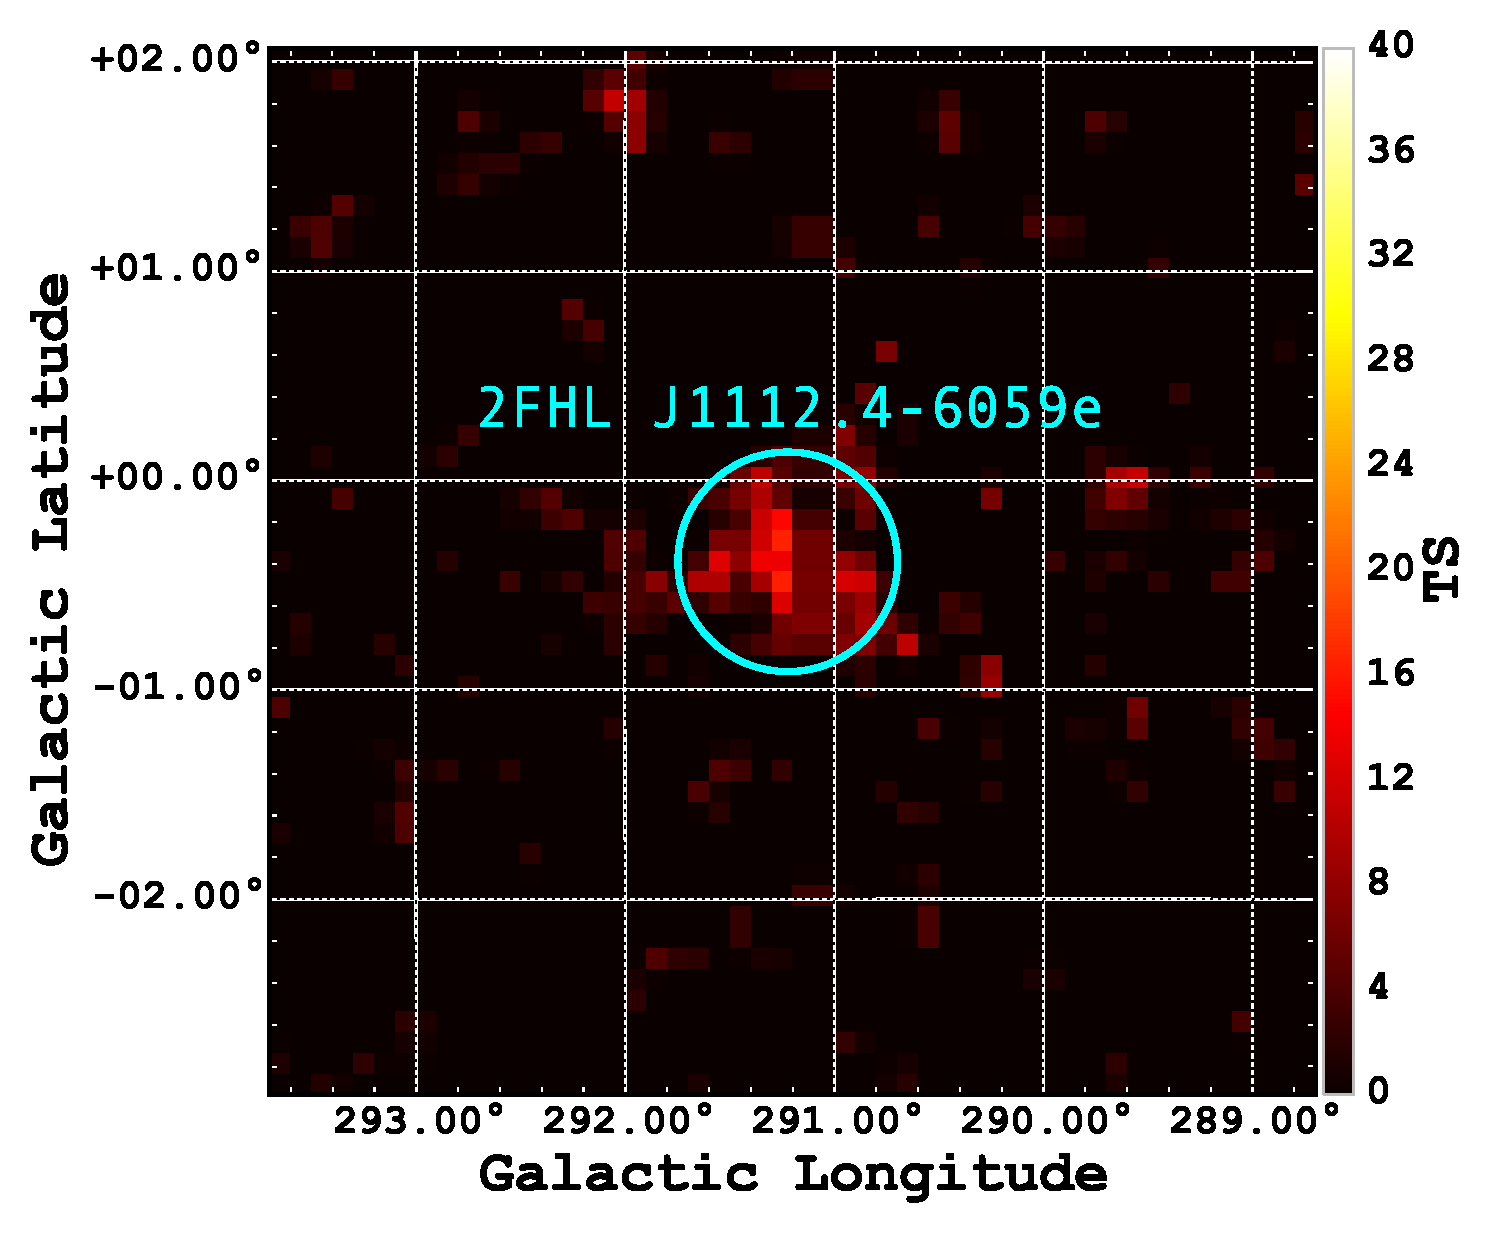
\includegraphics[width=8cm]{Figures/l290_b0_ES_1_residTSmap_2FHL_zoom.eps} \\
			\multicolumn{2}{c}{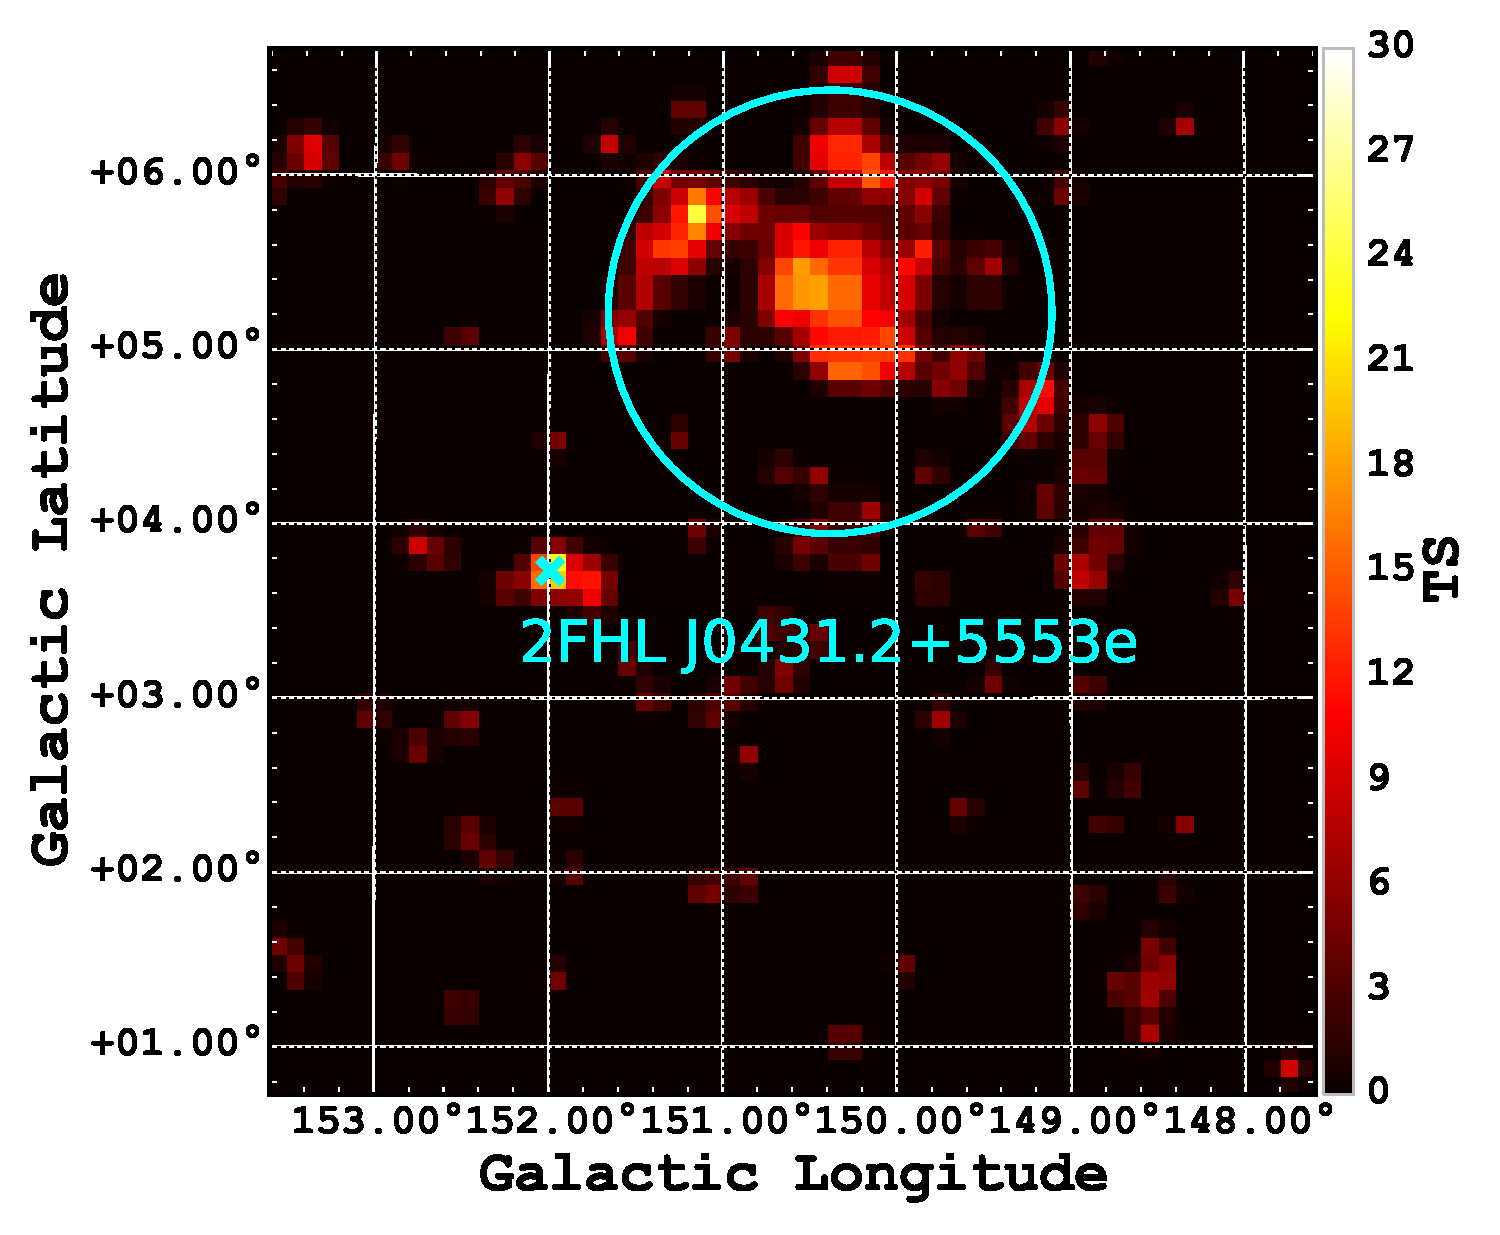
\includegraphics[width=8cm]{Figures/l145_b0_ES_1_residTSmap_2FHL_zoom.eps} }\\
		\end{tabular}
	\end{center}
	\caption{
		\label{fig:6ES} Residual TS maps for the five new extended sources described in Chapter \ref{2fhl:ESresults}.  Only the Galactic diffuse and isotropic emission are included in the model to highlight the location of emission not associated with the diffuse background. Circles indicate the extents of the fit disks. {The x marker in the bottom panel (2FHL~J0431.2+5553e) shows the location of a point source in the ROI.}}
\end{figure*}

\begin{deluxetable}{lccclccc}
\setlength{\tabcolsep}{0.04in}
\tablewidth{0pt}
\tabletypesize{\scriptsize}
\tcap{2FHL extended sources previously detected by the {\it Fermi}-LAT \label{tab:extended}}
\tablehead{
\colhead{2FHL Name} & 
\colhead{$l$ [deg]} & 
\colhead{$b$ [deg]} &
\colhead{TS} &
\colhead{Association} &
\colhead{Class} &
\colhead{Spatial model} &
\colhead{Radius [deg]}
}
\startdata
 J0526.6$-$6825e      &    278.843 &    -32.850 & 49.80  & LMC                & gal    & 2D Gaussian 		& 1.87 \\
 J0617.2+2234e        &    189.048 &      3.033 & 398.64 & IC~443             & snr    & 2D Gaussian 		& 0.27 \\
 J0822.6$-$4250e      &    260.317 &	 -3.277 &  63.87 & Puppis A	      & snr    & Disk	     		& 0.37 \\
 J0833.1$-$4511e      &    263.333 &     -3.104 & 49.70  & Vela~X             & pwn    & Disk        		& 0.91 \\
 J0852.8$-$4631e      &    266.491 &     -1.233 & 437.21 & Vela~Jr            & snr    & Disk        		& 1.12 \\
 J1303.4$-$6312e      &    304.235 &     -0.358 & 56.06  & HESS~J1303$-$631   & pwn    & 2D Gaussian 		& 0.24 \\
 J1514.0$-$5915e      &    320.269 &     -1.276 & 165.51 & MSH~15$-$52        & pwn    & Disk        		& 0.25 \\
 J1615.3$-$5146e      &    331.659 &     -0.659 & 128.15 & HESS~J1614$-$518   & spp    & Disk        		& 0.42 \\
 J1616.2$-$5054e      &    332.365 &     -0.131 & 87.18  & HESS~J1616$-$508   & pwn    & Disk        		& 0.32 \\
 J1633.5$-$4746e      &    336.517 &      0.121 & 114.17 & HESS~J1632$-$478   & pwn    & Disk        		& 0.35 \\
 J1713.5$-$3945e      &    347.336 &     -0.473 & 60.98  & RX~J1713.7$-$3946  & snr    & Map         		& 0.56 \\
 J1801.3$-$2326e      &      6.527 &     -0.251 & 50.20  & W~28               & snr    & Disk        		& 0.39 \\
 J1805.6$-$2136e      &      8.606 &     -0.211 & 160.43 & W~30               & snr    & Disk        		& 0.37 \\
 J1824.5$-$1350e      &     17.569 &     -0.452 & 266.09 & HESS~J1825$-$137   & pwn    & 2D Gaussian 		& 0.75 \\
 J1834.9$-$0848e      &     23.216 &     -0.373 &  67.30 & W~41               & spp    & 2D Gaussian		& 0.23 \\
 J1836.5$-$0655e      &     25.081 &      0.136 & 62.72  & HESS~J1837$-$069   & pwn    & Disk        		& 0.33 \\
 J1840.9$-$0532e      &     26.796 &     -0.198 & 163.15 & HESS~J1841$-$055   & pwn    & Elliptical 2D Gaussian & 0.62, 0.38, 39 \\
 J1923.2+1408e        &     49.112 &     -0.466 & 44.60  & W~51C              & snr    & Elliptical Disk        & 0.38, 0.26, 90 \\
 J2021.0+4031e        &     78.241 &      2.197 & 115.97 & Gamma Cygni        & snr    & Disk                   & 0.63 \\
 J2028.6+4110e        &     79.601 &      1.396 & 28.09  & Cygnus Cocoon      & sfr    & 2D Gaussian            & 3.0 \\
\enddata
\tablecomments{~List of the 20 extended sources in 2FHL that were previously detected as extended by the {\it Fermi}-LAT. All these sources are in  3FGL except W41, which is studied by \citet{W41}. The Galactic coordinates $l$ and $b$ are given in degrees. The extension of the disk templates is given by the radius. The extension of the 2D Gaussian templates is given by the $1\sigma$ radius, and the elliptical templates are given by the semi-major axis, semi-minor axis, and position angle (East of North). Association, Class, and Spatial model are as given in \threefgl{}.
}
\end{deluxetable}


\begin{deluxetable}{lcccccccclccc}
\setlength{\tabcolsep}{0.04in}
\tablewidth{0pt}
\tabletypesize{\scriptsize}
\tcap{New 2FHL extended sources 
\label{tab:new_extended}}
\tablehead{
\colhead{2FHL Name} & 
\colhead{$l$ [deg]} & 
\colhead{$b$ [deg]} &
\colhead{TS} & 
\colhead{TS$_{ext}$} &
\colhead{TS$_{2pts}$} &
\colhead{$F_{50}$} & 
\colhead{$\Delta F_{50}$} &
\colhead{$\Gamma$} & 
\colhead{$\Delta \Gamma$} &
\colhead{Association} &
\colhead{Class} &
\colhead{Radius [deg]} 
}
\startdata
 J0431.2+5553e        &    150.384 &      5.216 &  87.9 & 83.4  & 26.2    &  11.70 &       2.11 &    1.66 &         0.20 & G~150.3+4.5     & snr     & 1.27 $\pm$  0.04 \\
 J1112.4$-$6059e      &    291.222 &     -0.388 &  80.9 & 68.3   & 22.5    &  12.80 &       2.36 &    2.15 &         0.28 & PSR~J1112$-$6103  & pwn     & 0.53 $\pm$ 0.03 \\
 J1355.2$-$6430e      &    309.730 &     -2.484 &  82.3 & 31.8   & 12.9     &  9.59  &       1.95 &    1.56 &         0.22 & PSR~J1357$-$6429  & pwn     & 0.57 $\pm$ 0.02 \\
 %J1407.3$-$6116e      &    311.924 &      0.259 &  68.66 & 30.00       &  14.70 &       2.63 &    2.58 &         0.28 & \nodata         & \nodata & 0.38 \\
 J1419.2$-$6048e      &    313.432 &      0.260 & 109.3 & 49.1   & 15.6    &  17.60 &       2.80 &    1.87 &         0.19 & PSR~J1420$-$6048  & pwn     & 0.36 $\pm$ 0.03  \\
 J1443.2$-$6221e      &    315.505 &     -2.239 &  75.6 & 29.9   & 19.2   &  7.23  &       1.70 &    2.07 &         0.30 & SNR~G315.4$-$2.3  & snr     & 0.27 $\pm$  0.03 \\
\enddata
\tablecomments{~List of the 5 new extended sources in 2FHL. All sources are characterized by a uniform disk template whose radius and uncertainty therein is given in the last column. $l$ and $b$ are Galactic coordinates. All coordinates are shown in degrees. TS is the test statistic. ${\rm TS_{ext}} $ is the signicance of extension (\ref{2fhl:newES}). TS$_{2pts}$ is the TS of two simultaneously fit point sources  (\ref{2fhl:newES}). $F_{50}$ and $\Delta F_{50}$ are the integrated photon flux between 50~GeV and 2~TeV and its uncertainty in units of $10^{-11}$~photon~cm$^{-2}$~s$^{-1}$. $\Gamma$ and $\Delta \Gamma$ are the photon  index and its uncertainty from a power-law fit. Association lists the primary overlapping source and Class the suspected source type.  All uncertainties are $1\sigma$ uncertainties.}
\end{deluxetable}




%%%%%%


\section{\label{2FGL:summ}Summary} In this chapter, we have presented the publication on \twofhl, focusing primarily on the Galactic results of the publication and in particular detected extended sources. Extension of addSrcs to search for spatially extended sources, applied to 8 years \jamie{check} of LAT data above 50 \gev. Detected x extended. y were known 3FGL, z were new;y detected as extended at \gev~energies, \Gone ~was brand new. Galactic seem to have harder indices than extra gal, suggests which unid'd in the plane are gal vs. egal. All extended harder than diffuse. Hints of different morphology between \twofhl and \twofgl, didn't study here, but this is one of the motivations for $>$ 10 \gev study.
\section{Scratch}
Add stuff to first section about extension fitting with pointlike
In addition to being optimized for speed and large-scale studies (\ie{} those including many sources), \ptlike{}

I should probably give more detail about Josh's code than I did for just the regular pointlike?

Next, get into Josh's extension additions to pointlike
It accomplishes this by binning the sky in  

Should I say some things about why extension fitting is important in general?
